\documentclass[12pt]{report}
\usepackage[print,nopanel]{pdfscreen}
%\begin{print}
\usepackage{lipsum}% http://ctan.org/pkg/lipsum
\usepackage{titletoc}% http://ctan.org/pkg/titletoc
%\section{type}
\usepackage{sagetex}

\usepackage{lastpage}
\usepackage{macro/macro}
\usepackage{float}
\usepackage{fancyhdr}
\usepackage{verbatim}
\usepackage[Glenn]{fncychap}
\lhead{\large\bfseries Dynamics of Structure}
\usepackage[left=2.5cm, right=1.5cm, top=2.5cm, bottom=1.5cm]{geometry}
\pagestyle{fancy}
%\end{print}
\margins{0.5cm}{0.5cm}{0.5cm}{0.5cm}
\begin{screen}

\renewcommand{\encodingdefault}{T1}
\usepackage{setspace}
\linespread{1.5}
\renewcommand{\rmdefault}{ptm}
\end{screen}
\screensize{8cm}{9cm}
\overlay{overlay8.pdf}
\usepackage{graphicx}

\begin{document}
\newcommand{\centertext}[1]{\begin{center}\textbf{#1}\end{center}}
\newcommand{\student}{\vskip 2.5cm}
\newcommand{\supervisor}{\vskip 2cm}
\newcommand{\stamp}{\vskip 2.5cm}
\newcommand{\HRule}{\rule{\linewidth}{0.5mm}}
\newcommand{\projecttitle}{ \fontsize{24}{25}\selectfont \bf{Multi-Threaded Geometric Rendering}}
\newcommand{\tab}[1]{\hspace{.4\textwidth}\rlap{#1}}
\newcommand{\itab}[1]{\hspace{.05\textwidth}\rlap{#1}}
\newcommand{\logo}[1]{\includegraphics[scale=0.16]{#1}}
\newcommand{\submitted}{
\vskip 0.2in
\textnormal{ {\fontsize{14}{16}\selectfont \textbf{Project Report}} \\
	{\fontsize{12}{13}\selectfont of Major Project}\\
}
\vskip 0.2in

\textnormal{
 {\fontsize{14}{16}\selectfont \textbf{Bachelor of Technology}\\}
 {\fontsize{16}{17}\selectfont  (Computer Science and Engineering)\\}
}
\vskip 4cm
%\logo{images/gne.png}
%\image{0.7}{images/gne.png}{}

\includegraphics[width=7cm]{images/gne.png}
\vskip 2cm
\begin{minipage}{0.4\textwidth}
\begin{flushleft} \large
{Submitted by:}\\
\textnormal{{\fontsize{12}{13}\selectfont Amarjeet Singh Kapoor\\ D4CSE 2013-17 \\135005\\1311017 \\}} % Your name
\end{flushleft}
\end{minipage}
~
\begin{minipage}{0.4\textwidth}
\begin{flushright}
\textnormal{ \\
	 {\fontsize{12}{13}\selectfont Govind Sharma\\ D4CSE 2013-17 \\135026\\1311053\\}} % Supervisor's Name
\end{flushright}
\end{minipage}\\[1.5cm]
\HRule \\[0.4cm]

\textnormal{
Guru Nanak Dev Engineering College \\
Ludhiana 141006}
}


\newcommand{\pagetitle}{\begin{center}
\projecttitle
\Large\textbf{}\\
\submitted
\vskip 1cm

\end{center}}
\newcommand{\openoffice}{\textbf{OpenOffice}}
\newcommand{\frontmatter}[1]{\begin{Large} \textbf{#1} \end{Large}}
\newcommand{\ppttitle}{\begin{center}
\end{center}}

\begin{screen}
\ppttitle
\end{screen}
\footskip 0.7cm
\thispagestyle{empty} 
\pagetitle
\newpage
\pagenumbering{Roman}
\cfoot{\thepage}

\begin{Large}
\centertext{Acknowledgement}
\end{Large}

I, student of Guru Nanak Dev Engineering College, Ludhiana, have taken efforts in this project.
However, it would not have been possible without the kind support and help of many individuals
and organizations. I would like to extend my sincere thanks to all of them.\\

The author is highly grateful to Dr. M.S. Saini Director, Guru Nanak Dev Engineering College, Ludhiana for providing him with the opportunity to carry out his Six Weeks Training at
Testing and Consultancy Cell, Guru Nanak Dev Engineering College, Ludhiana.\\

The author would like to whole heartedly thank Dr. H.S. Rai Dean, Testing and Consultancy
Cell, Guru Nanak Dev Engineering College, Ludhiana who is a vast sea of knowledge and without whose constant and never ending support and motivation, it would never have been possible to complete the project and other assignments so efficiently and effectively.\\

Finally, I would thanks My Mentors at OpenSCAD organisation Marius Kintel and Torsten Paul. Without their encouragementand Guidence it would not have been possible to complete this project
in such an efficient manner.


\vskip 1.0cm 
\noindent Amarjeet Singh Kapoor

\newpage

%not compulsory

%\begin{Large}
\centertext{Abstract}
\end{Large}


User Interface for Customizing Models in OpenSCAD is the project that I worked upon for my 6-month training and also as Google summer of code project. It is under the umbrella organization of BRL-CAD. OpenSCAD is an open source organization that serves a free software to create solid 3d CAD objects. OpenSCAD has in a way redefined how easy 3D modeling can be. But the Wikipedia article on OpenSCAD says that it is a non-interactive modeler, but rather a 3D compiler based on a textual description language. Pay attention to the above line, it’s primarily what I’ll be talking about.

What the guys over at Wikipedia said is true but their version of the truth needs a little filtration (rather trimming). OpenSCAD’s way of customization is interactive, just not through a graphical interface. And this contingency makes the whole 3D modeling thing a little less easy than it can be. But all of that is about to change.

Solid 3D modeling. That sounds like some serious business. But it’s just an awesome tool for making models pertaining to many uses (mostly 3D printing). And 3D printing as we can all agree upon is cool. 3D models can be created by anyone using OpenSCAD. OpenSCAD is as much for designers as it is for you and me. What else can most people agree upon apart from the fact that solid 3D modeling is cool? A graphical interface is simpler and more intuitive to use. There is a general aversion for typing commands in order to get things done. Simply put, more people have an inclination towards GUI.

This is something that OpenSCAD lacked. But the benevolent folks at Thingiverse.com found a way to help out the demographic intersection of GUI lovers and OpenSCAD users. The website provides an easy to use interface to customize models of OpenSCAD. All one needs to do is upload the OpenSCAD file. After uploading the file, what you’ll see can only be described as being magic. I’m kidding, it’s just very useful is all. The OpenSCAD’s script is used to make a form containing slide bars, text boxes, combo boxes, labels, etc all for the singular purpose of customizing models.

My project was to include similar functionality into OpenSCAD itself. Constantly having to upload files created in one software (OpenSCAD) to a website in order to customize your models can get a little problematic as one is uploading scripts without being able to confirm how the script will translate into a form on the site. Wouldn’t it be great if everything is at one place, the original place: OpenSCAD? Of course, it would.

My project intends to define a user interface to customize models interactively instead of having to modify them manually. It will enable the user to create the templates for a given model which can further be changed as per user’s requirements.

This project will allow the modelers to create generic models (templates) which others can then customize to cater to their own use.

\newpage
\tableofcontents
\newpage
\listoffigures
\newpage
\listoftables
\newpage


\pagenumbering{arabic}
\cfoot{\thepage}

\newpage
\chapter{INTRODUCTION OF ORGANIZATION}
\begin{figure}[ht]
\centering
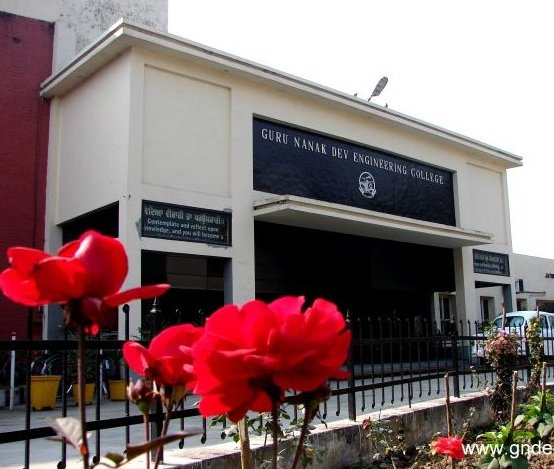
\includegraphics[scale=0.5]{images/gndec.jpg}
\caption{Guru Nanak Dev Engineering College}
\end{figure}
\hspace{-1.7em} I had my Six Month Industrial Training at TCC-Testing And Consultancy Cell, GNDEC Ludhiana. Guru Nanak Dev Engineering College was established by the Nankana
Sahib Education Trust Ludhiana. The Nankana Sahib Education Trust i.e NSET
was founded in memory of the most sacred temple of Sri Nankana Sahib, birth place
of Sri Guru Nanak Dev Ji. With the mission of Removal of Economic Backwardness
through Technology Shiromani Gurudwara Parbandhak Committee i.e SGPC started a
Poly technical was started in 1953 and Guru Nanak Dev Engineering College was established in 1956.\\


The main goal of this institute is:
\begin{itemize}
\item To build and promote teams of experts in the upcoming specialisations.
\item To promote quality research and undertake research projects keeping in view their
relevance to needs and requirements of technology in local industry.
\item To achieve total financial independence.
\item To start online transfer of knowledge in appropriate technology by means of establishing multipurpose resource centres.
\end{itemize}
\section{Testing and Consutancy Cell}

I had my Six Month Institutional Training at TCC i.e Testing And
Consultancy Cell,
GNDEC Ludhiana under the guidance of Dr. H.S.Rai Dean Testing and Consultancy Cell.
Testing and Consultancy Cell was established in the year 1979 with a basic aim to produce
quality service for technical problems at reasonable and affordable rates as a service to society
in general and Engineering fraternity in particular.\\
\begin{figure}[ht]
\centering
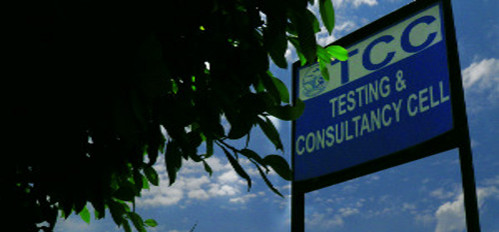
\includegraphics[scale=0.7]{images/aw.jpg}
\caption{Testing and Consultancy Cell}
\end{figure}
\hspace{-1.7em} 

Consultancy Services are being rendered by various Departments of the College to the
industry, Sate Government Departments and Entrepreneurs and are extended in the form of
expert advice in design, testing of materials \& equipment, technical surveys, technical audit,
calibration of instruments, preparation of technical feasibility reports etc.
This consultancy cell of the college has given a new dimension to the development
programmers of the College. Consultancy projects of over Rs. one crore are completed by the
Consultancy cell during financial year 2009-10. \\

Ours is a pioneer institute providing Consultancy Services in the States of Punjab, Haryana,
Himachal, J\&K and Rajasthan. Various Major Clients of the Consultancy Cell are as under:\\
\begin{itemize}
\item Northern Railway, Govt. of India
\item Indian Oil Corporation Ltd.
\item Larson \& Turbo.
\item Multi National Companies like AFCON \& PAULINGS.
\item Punjab Water Supply \& Sewage Board
\end{itemize}


\newpage
%\chapter{\LaTeX}
%\section{Introduction to \LaTeX}

\LaTeX, I had never heard about this term before doing this project,
but when I came to know about it's features, found it excellent. 
\LaTeX{} (pronounced /ˈleɪtɛk/, /ˈleɪtɛx/, /ˈlɑːtɛx/, or /ˈlɑːtɛk/) is a 
document markup language and document preparation system for the \TeX{} 
typesetting  program. Within the typesetting system, its name is styled 
as \LaTeX.

\image{0.9}{images/donald.png}{Donald Knuth, Inventor Of \TeX{} 
typesetting system}

Within the typesetting system, its name is styled as \LaTeX. The term 
\LaTeX{} refers only to the language in which documents are written, 
not to the editor used to write those documents. In order to create a 
document in \LaTeX, a .tex file must be created using some form of text 
editor. While most text editors can be used to create a \LaTeX{} document, 
a number of editors have been created specifically for working with \LaTeX.

\LaTeX{} is most widely used by mathematicians, scientists, 
engineers, philosophers, linguists, economists and other scholars in 
academia. As a primary or intermediate format, e.g., translating DocBook 
and other XML-based formats to PDF, \LaTeX{} is used because of the 
high quality of typesetting achievable by \TeX. The typesetting system 
offers programmable desktop publishing features and extensive facilities 
for automating most aspects of typesetting and desktop publishing, 
including numbering and cross-referencing, tables and figures, 
page layout and bibliographies.

\LaTeX{} is intended to provide a high-level language that
accesses the power of \TeX. \LaTeX{} essentially comprises a
collection of \TeX{} macros and a program to process \LaTeX documents. 
Because the \TeX{} formatting commands are very low-level, it is usually 
much simpler for end-users to use \LaTeX{}.


\subsection{Typesetting}
\LaTeX{} is based on the idea that authors should be able to focus on 
the content of what they are writing without being distracted by its 
visual presentation. In preparing a \LaTeX{} document, the author 
specifies the logical structure using familiar concepts such as 
chapter, section, table, figure, etc., and lets the \LaTeX{} system 
worry about the presentation of these structures. It therefore 
encourages the separation of layout from content while still allowing 
manual typesetting adjustments where needed. 

\begin{verbatim}
\documentclass[12pt]{article}
\usepackage{amsmath}
\title{\LaTeX}
\date{}
\begin{document}
  \maketitle 
  \LaTeX{} is a document preparation system 
  for the \TeX{} typesetting program.
   \par 
   $E=mc^2$
\end{document}
\end{verbatim}


\chapter{Introduction To Project}

% pending 
\section{Overview}
Dynamics of Structures (DoS) is an open-source, free web-based software, developed by students of 
Testing and Consultancy Cell (TCC), under the guidance of Dr. H.S. Rai. This software is used to compute the 
Modes of vibration in which the structure can move and also force applied on each floor 
due to the vibration caused by the earthquake. So, that Civil engineers can
analysis the stability of structure consisting of many stories.

 The main task of this application is to get data as input from user and then it can compute 
the result at back-end and when the result is ready it send output as email.
This software is structured by keeping in view that user of this software can be both 
a Civil Engineer or a simple man whose job is just to enter data to software 
in order that an engineer can analyze later from the result stability of the structure.
This software also provides the intermediate values for engineering student 
to deeply analyze the process of computation to be done in order to get output values.


The core part of DoS is implemented using Sagemath for processing,  \LaTeX{} for output file (PDF) generation, django 
for web interface. Bash Shell Scripting has been used to join all these. To provide the User Experience to the users, 
Bootstrap has been used.


My training being not based on particular language or technology, different type of open-source softwares and technologies are 
used in this project and many during my training which are not used in this 
project like OpenCV (for image processing and computer vision), CGI (for web interface through c++).


%%%% This include existing system and will include user requirement
\section{The Existing System}
There are few existing systems for solving this particular problem like STAAD.Pro, SAP2000 but they don't have
following features required by our mentor. These system were not open source and free web based software 
that were need.


All exiting system suffers from at least one of the following system.  



{\bf {Limitations of previous system }}
\begin{itemize}
\item No batch mode 

\item Don't give output as PDF

\item They are costly ( STAAD.Pro costs nearly 80,000 rupees )

\item They don't mail output 

\item They need installation and a lot of system resources 

\item They don't accept values in form of *.csv file 
\end{itemize}



\section{User Requirement Analysis} 
For User Requirement Analysis, users of this system have been asked about 
possible requirements that this software should have and we got following
resultant list of outputs-:
\begin{enumerate}
\item Generates the final output in the form of pdf
\item Provide on-line way to analysis so that individual does not have to 
install anything.
\item Send PDF to the user in the form of email
\item Make it work like batch mode. so, that user can give inputs 
together and relax.
\item Accept inputs from the user in *.csv file format
\item Help M.Tech and Civil Engineer to analysis structure.
\item Automate calculation of modal force and modes.
\item Reduce the time for analysis.
\end{enumerate}


\section{Feasibility Analysis}
Feasibility analysis aims to uncover the strengths and weaknesses of 
a project. In its simplest term, the two criteria to judge feasibility 
are cost required and value to be attained. As such, a well-designed 
feasibility analysis should provide a historical background of the 
project, description of the project or service, details of the 
operations and management and legal requirements. Generally, feasibility 
analysis precedes technical development and project implementation. 
There is some feasibility factors by which we can determine that 
project is feasible or not:
\begin{itemize}
\item {\bf{Technical feasibility}}: Technological feasibility is carried 
out to determine whether the project has the capability, in terms of 
software, hardware, personnel to handle and fulfill the user 
requirements. This whole project is based on solving Mathematics equations for which we have used SAGEMATH and to provide output we have used \LaTeX{} for providing the output and Django for user interface. Technical feasibility of this project revolves around the technical boundaries and limitations of the SAGEMATH, \LaTeX{} and Django. But as \LaTeX{} is much powerful Typesetting tool and Django is secure and structured server side framework, so these languages and technologies are perfect to design the software under this project. Dynamics of sturcture is technically feasible as it is built up in Open 
Source Environment and thus it can be run on any Open Source platform.
\item {\bf{Economic feasibility}}: Economic analysis is the most 
frequently used method to determine the cost/benefit factor for 
evaluating the effectiveness of a new system. In this analysis we 
determine whether the benefit is gain according to the cost invested 
to develop the project or not. If benefits outweigh costs, only then 
the decision is made to design and implement the system. It is 
important to identify cost and benefit factors, which can be categorized 
as follows:
\begin{enumerate}
\item Development costs.
\item Operating costs.
\end{enumerate}
Dynamics of structure Software is also Economically feasible with 0 Development 
and Operating Charges as it is developed in Django framework, SAGEMATH and \LaTeX{}  which is FOSS technology and the software is operated on Open 
Source platform.
\item {\bf{Operational feasibility}}: Operational feasibility is a measure 
of how well a project solves the problems, and takes advantage of the 
opportunities identified during scope definition and how it satisfies 
the requirements identified in the requirements analysis phase of system 
development. All the Operations performed in the software are very quick 
and satisfies all the reuirements. This project is also operational feasible as it automates the work of solving the problem of analysising the structures which not only saves time but also saves money as most of the work is done by Employees and M.Tech students is done by this software.
\end{itemize}




\section{Objective of Project}
Dynamic of structure is a web based software and the 
main objectives of this project is to -:
\begin{enumerate}
\item To inspire M.Tech students to automate their work and do programming 
\item Perform most of difficult Calculation work.
\item Make it work like batch mode. so, that user can give inputs 
together and relax.
\item Accept inputs from the user in *.csv file format
\item Help M.Tech and Civil Engineer to analysis structure.
\item Automatic calculation of modal force and modes.
\item Reduce the time for analysis.
\item Generates the final output in the form of pdf
\item Provide on-line way to analysis so that individual does not have to 
install anything.
\item Send PDF to the user in the form of email.
\end{enumerate}

\chapter{PROJECT DESIGN}
\section{Software Requirement Analysis}

A Software Requirements Analysis for a software system is a complete 
description of the behavior of a system to be developed. It include functional Requirements
and Software Requirements. In addition to these, the SRS also contains 
non-functional requirements. Non-functional requirements are 
requirements which impose constraints on the design or implementation.
\begin{itemize}
\item{\bf Purpose}: Dynamic of structure is a web based software and the 
main purpose of this project is to:
\begin{enumerate}
\item Perform most of difficult Calculation work.
\item Make it work like batch mode. so, that user can give inputs 
together and relax.
\item Help M.Tech and Civil Engineer to analysis structure.
\item Automatic calculation of modal force and modes.
\item Reduce the time for analysis.
\item Provide on-line way to analysis so that individual does not have to 
install anything.
\end{enumerate}

\item{\bf Users of the System}
\begin{enumerate} 
\item Client : Clients are the end users that benefit from this software.
They just provide input and gets output in form of PDF.Client of this 
WEB Application can be of two types -:
\begin{enumerate}
\item Civil Engineer -: They have knowledge of working of procedure
and what input is being provided.
\item Layman -: They don't know anything about what's going on, their just 
work is to give input to system.   
 
\end{enumerate}
\end{enumerate}
\end{itemize}

\subsection{Functional Requirements}
\begin{itemize}
\item {\bf Specific Requirements}: This phase covers the whole requirements 
for the system. After understanding the system we need the input data 
to the system then we watch the output and determine whether the output 
from the system is according to our requirements or not. So what we have 
to input and then what we’ll get as output is given in this phase. This 
phase also describe the software and non-function requirements of the 
system.
\item {\bf Input Requirements of the System}
\begin{enumerate} 
\item Type of soil
\item Number of storeys
\item Importance Factor
\item Response Reduction Factor
\item Zone Factor
\item Input method (CSV or manual)
\item Output method (Email or direct PDF)
\item Mass of each storey
\item Height of each storey
\item Stiffness of each storey
\item Input in form of csv file
\end{enumerate}
\vskip 0.5cm
\item {\bf Output Requirements of the System}
\begin{enumerate} 
\item Calculation of modal force and modes.
\item Generation of output in form of PDF.
\item Mailing output PDF 
\end{enumerate}
\vskip 0.5cm
\item {\bf Special User Requirements}
\begin{enumerate} 
\item Automatic Email Generation of Output and Sending to the concerned person.
\item Taking bulk input values in form of CSV file
\end{enumerate}
\vskip 0.5cm
\item {\bf Software Requirements}
\begin{enumerate} 
\item Programming language: Python 2.7
\item software: SAGEMATH, \LaTeX{}
\item Framework: Django 1.7, Bootstrap
\item Web Languages: Html, Java Script, CSS
\item Database: Sqlite 
\item Documentation: Doxygen 1.8.3
\item Text Editor: Vim
\item Operating System: Ubuntu 12.04 or up
\item Revision System: Git

\end{enumerate}
\vskip 0.5cm
\subsection{Non functional requirements}
\begin{enumerate} 
\item Scalability: System should be able to handle a number of users. 
For e.g., handling around thousand users at the same time.
\item Usability: Simple user interfaces that a layman can understand.
\item Speed: Processing input should be done in reasonable time
 i.e. we can say maximum 24 hrs.
\end{enumerate}
\end{itemize}




\section{Flowchart}
A flowchart is a type of diagram that represents an algorithm, work flow or process, showing the steps as boxes of various kinds, and their order by connecting them with arrows
and the flowchart \ref{fig:FD1} of customizer showing the flow of control and Data in the software.

\begin{figure}
	\centering 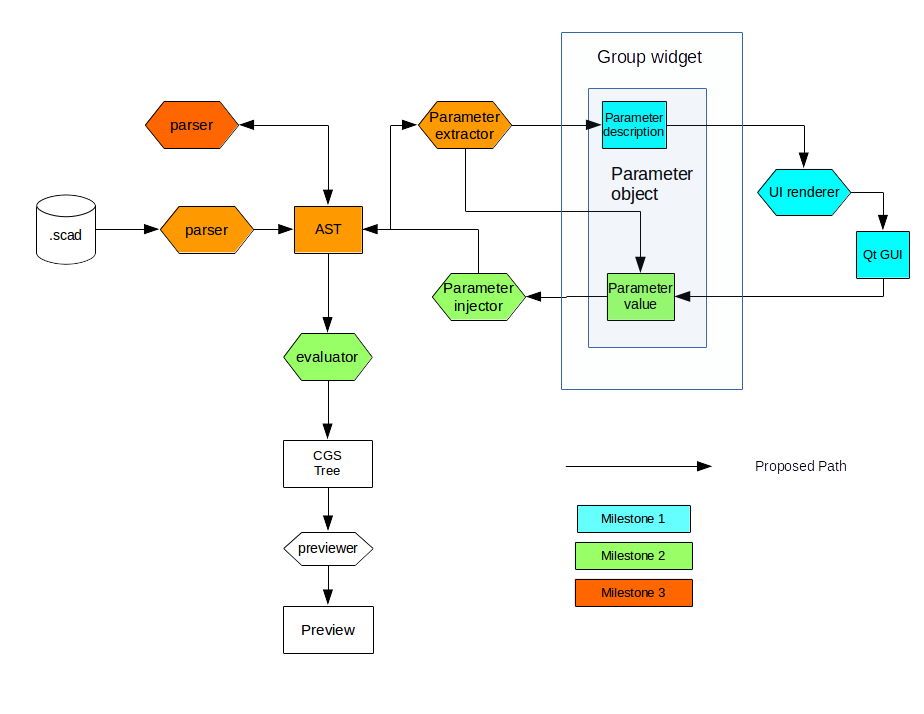
\includegraphics[width=\linewidth]{images/flowchart.png}
	\caption{Flowchart of Customizer}
	\label{fig:FD1}
\end{figure}

\subsection{Detailed Description}

The basic implementation of this project is almost done in form of prototype. There is need to modify the structure of the project. We have to divide the task into there parts:

\begin{enumerate}
	\item \textbf{Front end}
	It will deal with how the parameter will look to the user like in form of range or spinbox etc. This part will include two parts:
	\begin{enumerate}
		\item \textbf{Individual Parameter}
		This will define how individual parameters will look like
		\item \textbf{Container Widget}
		This will contain UI features common to all parameter. This widget will contain all parameter widget.
		
	\end{enumerate}
	
	\item \textbf{Back End}
	This will include the parser part that will create AST nodes and we can extract the parameters from the AST. we can use the single parser for the whole .scad file or separate parser for extracting the parameters with annotations.
	
	The Back-end part will also include the parameter extractor and injector or the injector can be included in parameter object which will serve as interface
	\item \textbf{Interface}
	This will include the parameter object which will serve as an interface between both Back end and Front end. Parameter object will contain information regarding each individual parameter like parameter name, default value, and information how this parameter will be displayed as widgets to the user. Parameter object could also include the method to inject the value of the individual parameter into the AST.
	
\end{enumerate}


\section{Dependency Graph}
A Dependency Graph is a graphical representation of the which module is dependent on which other modules. A Dependency Graph is often used as a preliminary step to creating an overview of the system. Dependency Graph also gives overview of how good is the design of the system.
OpenSCAD being were huge software it would be difficult to make the dependency graph of whole software. So, here is  Dependency Graph of Customizer is as following-:
\begin{enumerate}
\item \textbf{Dependency graph of Comment.h:} Figure \ref{fig:comment1} shows the modules on which the comment.h module is dependent.
\item \textbf{Caller graph of Comment.h:} Figure \ref{fig:comment} shows the modules that use the module comment.h.
\item \textbf{Caller graph of ParameterWidget.cc:} Figure \ref{fig:dependency} show the modules that uses the module ParameterWidget.h.
\end{enumerate}

\begin{figure}
	\centering
	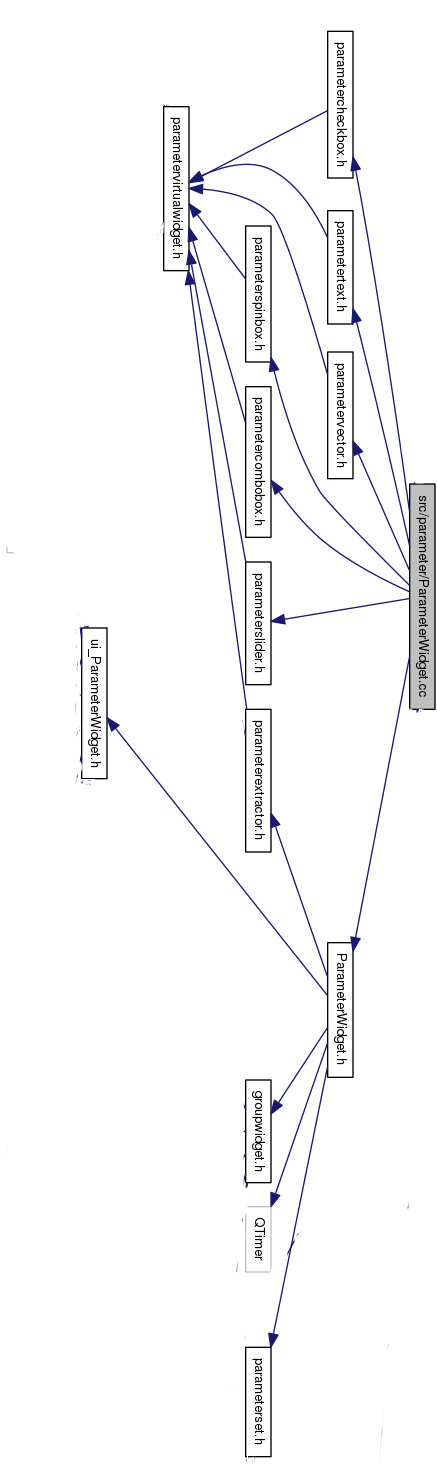
\includegraphics[width=0.7\linewidth,height=1.37\columnwidth]{images/dependene}
	\caption{ Dependency graph of Comment.h}
	\label{fig:dependency}
\end{figure}

\begin{figure}
\centering
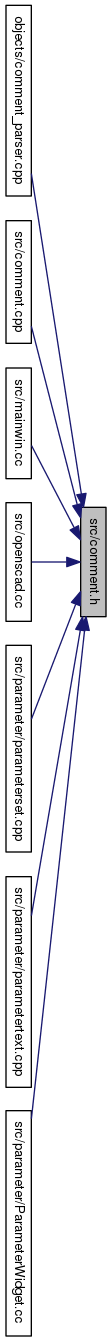
\includegraphics[width=0.25\linewidth,height=1.37\columnwidth]{images/comment}
\caption{Caller graph of Comment.h}
\label{fig:comment}
\end{figure}
\begin{figure}
\centering
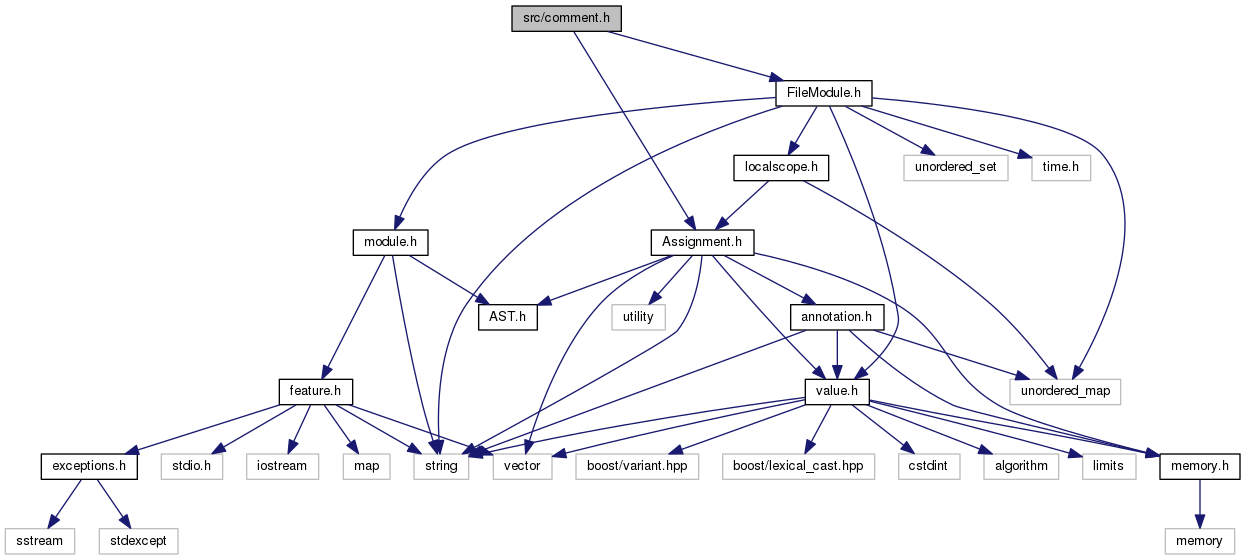
\includegraphics[width=\linewidth,height=1.35\columnwidth]{images/comment1}
\caption{Caller graph of ParameterWidget.cc}
\label{fig:comment1}
\end{figure}




\section{Class Diagrams}
Class Diagrams describe the static structure of the system. Following classes diagram represent the relationship between different classes in OpenSCAD and customizer:
\begin{enumerate}
	\item Figure \ref{fig:collaborative1} shows the class diagram of the ParameterWidgetVirtual class which is the basse class of all the Widget classes i.e ParameterCheckbox, ParameterVector,ParmeterSpinbox, ParameterComboBox,ParameterSlider, ParameterText.
	\item Figure \ref{fig:collaborative} shows the class diagram of the ParameterWidget class which is the main class for whole the Customizer GUI and also show how this class is related to various classes in custmoizer.
	
	\item Figure \ref{fig:classAnnotation__coll__graph}  shows the class diagram of the Annotation class which is the main node of the AST that support the customizer feature and also show how this class is related to various classes in the customizer.
\end{enumerate}
\begin{figure}
    \centering
    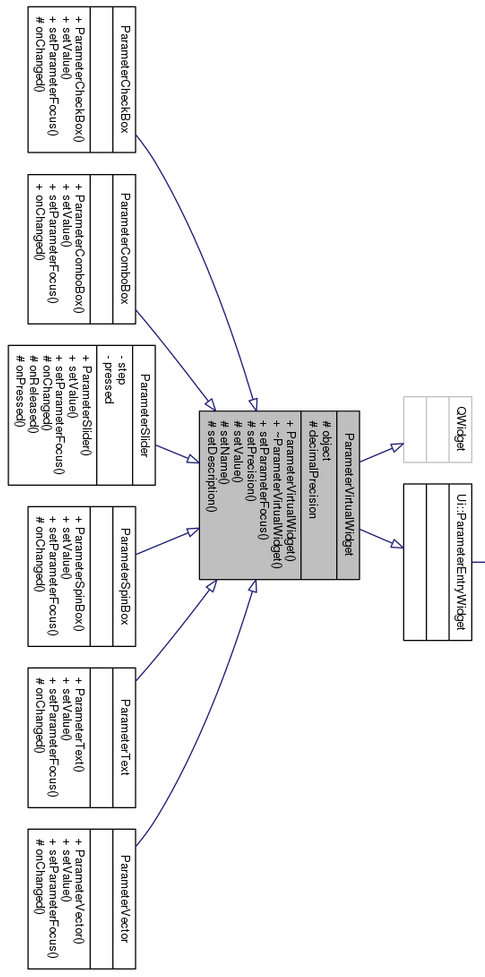
\includegraphics[width=0.5\linewidth,,height=1.38\columnwidth]{images/collaborative1}
    \caption{Class Diagram for Customizer (Part A) }
    \label{fig:collaborative1}
\end{figure}
\begin{figure}
    \centering
    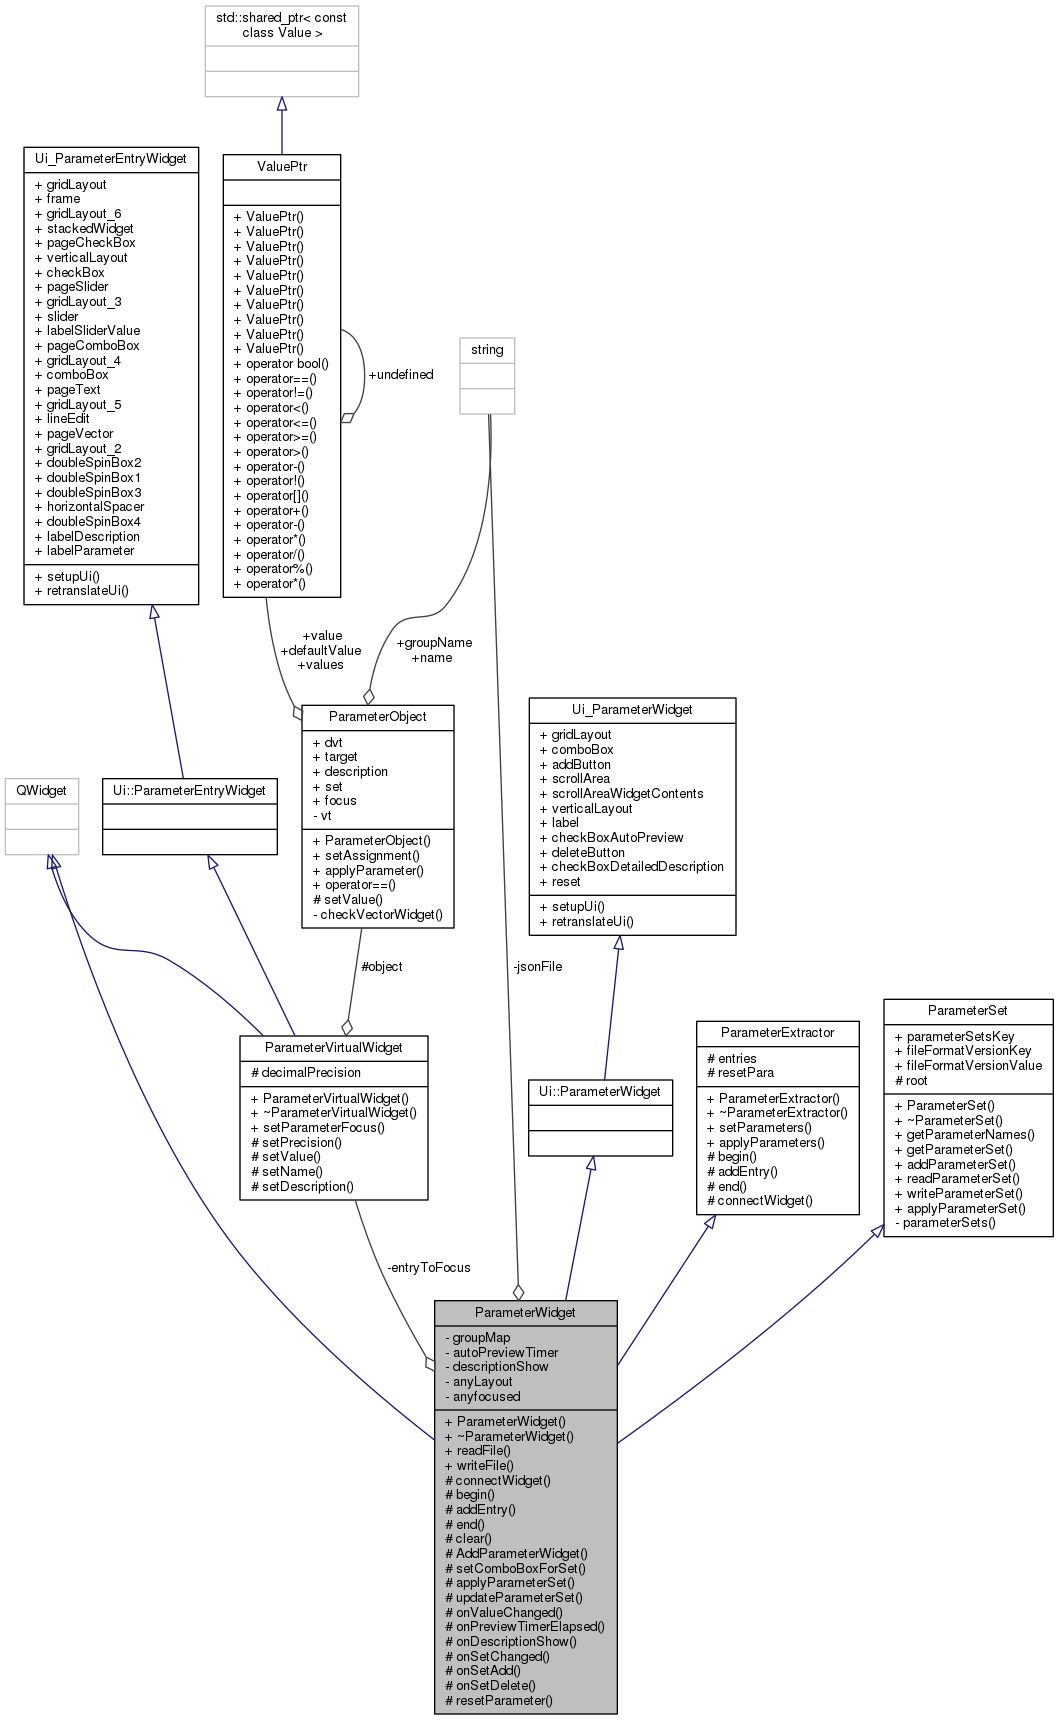
\includegraphics[scale=0.39]{images/collaborative}
    \caption{Class Diagram for Customizer (Part B)}
    \label{fig:collaborative}
\end{figure}
\begin{figure}
\centering
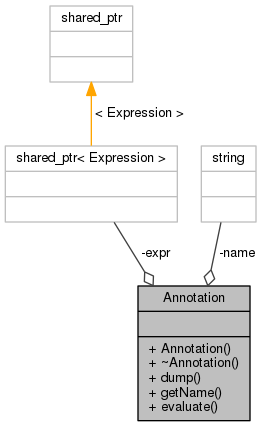
\includegraphics[width=0.4\linewidth]{images/classAnnotation__coll__graph}
\caption{Class Diagram for Annotation}
\label{fig:classAnnotation__coll__graph}
\end{figure}
\section{Dependencies}
Dependencies include softwares or framework that need to be installed for 
proper working of this software.

\begin{enumerate} 
\item Programming language: Python 2.7
\item Software: SAGEMATH, \LaTeX{}
\item Framework: Django 1.7
\item Operating System: Any on which above dependencies can be installed
\end{enumerate}







\newpage
\chapter{DEVELOPMENT AND IMPLEMENTATION}
\section{Python} 
\begin{figure}[h]
\centering 
\includegraphics[scale=0.3]{images/python.jpg}
\caption{Python logo}
\end{figure}
\noindent Python is a dynamic language, as in python coding is very easy and 
also it require less coding and about its interpreted nature it is 
just exellent. Python is a high level programming language and Django 
which is a web development framework is written in python language.

Python is an easy to learn, powerful programming language.Python runs 
on Windows, Linux/Unix, Mac OS X. Python is free to use, even for 
commercial products. Python can also be used as an extension language 
for existing modules and applications that need a programmable interface.  
Python is free to use, even for commercial products, because of its 
OSI-approved open source license.
\subsection{Features of Python}
\begin{itemize}
\item Very clear, readable syntax.
\item Strong introspection capabilities.
\item Intuitive object orientation.
\item Natural expression of procedural code.
\item Full modularity, supporting hierarchical packages.
\item Exception-based error handling.
\item Very high level dynamic data types.
\item Extensive standard libraries and third party modules for virtually every task.
\item Extensions and modules easily written in C, C++ (or Java for Jython, or .NET languages for IronPython).
\item Embeddable within applications as a scripting interface.
\end{itemize}
\subsection{Installation of Python}
Installation of python is a very easy proccess.
The current python versions are: Python 2.7.1 and Python 3.2.
Type the commands in the terminal:\\

 \$ wget http://www.python.org/ftp/python/2.7/Python-2.7.tgz\\

 
 \$ tar xzf Python-2.7.tgz\\


This will install the python on your pc/laptop.





\section[Front End Languages and Framework]{Front End Languages 
and Framework \footnote{ Used in project but not by me accept 
basic HTML}}

Front End languages are language that are used to give better user experince and user interface. These mainly include HTML, CSS, Javascript. Some Frameforks like Bootstrap are also used with these basic languages.
\subsection{HTML}

\begin{figure}[h]
\centering 
\includegraphics[scale=0.05]{images/HTML.png}
\caption{HTML5 logo}
\end{figure}
HyperText Markup Language, commonly referred to as HTML, is the standard markup language used to create web pages. Along with CSS, and JavaScript, HTML is a cornerstone technology, used by most websites to create visually engaging webpages, user interfaces for web applications, and user interfaces for many mobile applications. Web browsers can read HTML files and render them into visible or audible web pages. HTML describes the structure of a website semantically along with cues for presentation, making it a markup language, rather than a programming language.


HTML elements form the building blocks of all websites. HTML allows images and objects to be embedded and can be used to create interactive forms. It provides a means to create structured documents by denoting structural semantics for text such as headings, paragraphs, lists, links, quotes and other items.

\begin{verbatim}
<!DOCTYPE html>
<html>
  <head>
    <title>This is a title</title>
  </head>
  <body>
    <p>Hello world!</p>
  </body>
</html>

\end{verbatim}


\subsection{CSS}

\begin{figure}[h]
\centering 
\includegraphics[scale=0.50]{images/CSS.jpg}
\caption{CSS logo}
\end{figure}
Cascading Style Sheets (CSS) is a style sheet language used for describing the presentation of a document written in a markup language.Although most often used to set the visual style of web pages and user interfaces written in HTML and XHTML, the language can be applied to any XML document, including plain XML, SVG and XUL, and is applicable to rendering in speech, or on other media. Along with HTML and JavaScript, CSS is a cornerstone technology used by most websites to create visually engaging webpages, user interfaces for web applications, and user interfaces for many mobile applications.


CSS is designed primarily to enable the separation of document content from document presentation, including aspects such as the layout, colors, and fonts. This separation can improve content accessibility, provide more flexibility and control in the specification of presentation characteristics, enable multiple HTML pages to share formatting by specifying the relevant CSS in a separate .css file, and reduce complexity and repetition in the structural content, such as semantically insignificant tables that were widely used to format pages before consistent CSS rendering was available in all major browsers. CSS makes it possible to separate presentation instructions from the HTML content in a separate file or style section of the HTML file. For each matching HTML element, it provides a list of formatting instructions

\begin{verbatim}
p {
    color: red;
    text-align: center;
} 
\end{verbatim}

\subsection{Javascript}
\begin{figure}[h]
\centering 
\includegraphics[scale=0.3]{images/JS.png}
\caption{Javascript logo}
\end{figure}
JavaScript (/ˈdʒɑːvəˌskrɪpt/) is a high-level, dynamic, untyped, and interpreted programming language. It has been standardized in the ECMAScript language specification. Alongside HTML and CSS, it is one of the three essential technologies of World Wide Web content production; the majority of websites employ it and it is supported by all modern web browsers without plug-ins. JavaScript is prototype-based with first-class functions, making it a multi-paradigm language, supporting object-oriented, imperative, and functional programming styles. It has an API for working with text, arrays, dates and regular expressions, but does not include any I/O, such as networking, storage or graphics facilities, relying for these upon the host environment in which it is embedded.

\subsection{BootStarp} 
\begin{figure}[h]
\centering 
\includegraphics[scale=0.2]{images/boot.png}
\caption{BootStrap logo}
\end{figure}

Bootstrap is a free and open-source collection of tools for creating websites and web applications. It contains HTML and CSS-based design templates for typography, forms, buttons, navigation and other interface components, as well as optional JavaScript extensions. It aims to ease the development of dynamic websites and web applications.

Bootstrap is a front end framework, that is, an interface for the user, unlike the server-side code which resides on the "back end" or server.




\section{Shell Scripting}
Normally shells are interactive. It means shell accept command from you (via keyboard) and execute them. But if you use command one by one (sequence of 'n' number of commands) , the you can store this sequence of command to text file and tell the shell to execute this text file instead of entering the commands. This is know as shell script.
Shell script defined as series of command written in plain text file. Shell script is just like batch file is MS-DOS but have more power than the MS-DOS batch file.
why to Write Shell Script ?
\begin{enumerate} 
\item Shell script can take input from user, file and output them on screen.
\item Useful to create our own commands.
\item Save lots of time.
\item To automate some task of day today life.
\item System Administration part can be also automated.
\end{enumerate} 
{ \bf Execute your script as syntax:}
\begin{verbatim}
chmod 755 your-script-name
sh your-script-name
./your-script-name
\end{verbatim}

\section{Introduction to \LaTeX}

\LaTeX, I had never heard about this term before doing this project,
but when I came to know about it's features, found it excellent. 
\LaTeX{} (pronounced /ˈleɪtɛk/, /ˈleɪtɛx/, /ˈlɑːtɛx/, or /ˈlɑːtɛk/) is a 
document markup language and document preparation system for the \TeX{} 
typesetting  program. Within the typesetting system, its name is styled 
as \LaTeX.

\image{0.9}{images/donald.png}{Donald Knuth, Inventor Of \TeX{} 
typesetting system}

Within the typesetting system, its name is styled as \LaTeX. The term 
\LaTeX{} refers only to the language in which documents are written, 
not to the editor used to write those documents. In order to create a 
document in \LaTeX, a .tex file must be created using some form of text 
editor. While most text editors can be used to create a \LaTeX{} document, 
a number of editors have been created specifically for working with \LaTeX.

\LaTeX{} is most widely used by mathematicians, scientists, 
engineers, philosophers, linguists, economists and other scholars in 
academia. As a primary or intermediate format, e.g., translating DocBook 
and other XML-based formats to PDF, \LaTeX{} is used because of the 
high quality of typesetting achievable by \TeX. The typesetting system 
offers programmable desktop publishing features and extensive facilities 
for automating most aspects of typesetting and desktop publishing, 
including numbering and cross-referencing, tables and figures, 
page layout and bibliographies.

\LaTeX{} is intended to provide a high-level language that
accesses the power of \TeX. \LaTeX{} essentially comprises a
collection of \TeX{} macros and a program to process \LaTeX documents. 
Because the \TeX{} formatting commands are very low-level, it is usually 
much simpler for end-users to use \LaTeX{}.


\subsection{Typesetting}
\LaTeX{} is based on the idea that authors should be able to focus on 
the content of what they are writing without being distracted by its 
visual presentation. In preparing a \LaTeX{} document, the author 
specifies the logical structure using familiar concepts such as 
chapter, section, table, figure, etc., and lets the \LaTeX{} system 
worry about the presentation of these structures. It therefore 
encourages the separation of layout from content while still allowing 
manual typesetting adjustments where needed. 

\begin{verbatim}
\documentclass[12pt]{article}
\usepackage{amsmath}
\title{\LaTeX}
\date{}
\begin{document}
  \maketitle 
  \LaTeX{} is a document preparation system 
  for the \TeX{} typesetting program.
   \par 
   $E=mc^2$
\end{document}
\end{verbatim}



\section{Introduction to Django}
\begin{figure}[h]
\centering 
\includegraphics[scale=0.13]{images/django.png}
\caption{Django logo}
\end{figure}
\noindent Django is an open source web application framework written in python. It lets 
you build high-performing, elegant Web applications quickly. Django 
focuses on automating as much as possible. Django's primary goal is to 
ease the creation of complex, database-driven websites. Django 
emphasizes reusability and "pluggability" of components, rapid 
development, and the DRY principal. Python is used throughout, even 
for settings, files, and data models. Django also provides an optional
 administrative create, read, update and delete interface that is 
generated dynamically through introspection and configured via admin 
models.

Django takes it's name from the early jazz guitarist Django Reinhardt, 
a gypsy savant who managed to play dazzling and electrifying runs on 
his instrument even though two of the fingers on his left hand were 
paralyzed in an accident when he was young.

Thus it’s a fitting name for the framework. Django can do some very 
complex things with less code and a simpler execution than you’d expect. 
It doesn't take a heavy hand to build with Django. The framework does 
the repetitive work for you, allowing you to get a working website up 
quickly and easily.
\subsection{Features of Django}
\begin{itemize}
\item Clean URLs
\item Object- Relational Mapping
\item Loosely coupled components
\item Designer-friendly templates  
\item Cache framework 
\item MVC architecture
\item Jython support
\item DRY ( Don't Repeat Yourself)
\end{itemize}
\subsection{Installation of Django}
Installation of Django is very easy. To install Django version 1.4,
type the following commands:\\

	\$ wget http://www.djangoproject.com/download/1.4/tarball\\


	\$ tar xzvf Django-1.4.tar.gz\\


	\$ cd Django-1.4\\


	\$ sudo python setup.py install \\

\noindent This will install the django on your system.
 
\noindent \subsection{MTV} Django adopts the standard 
MVC (Model-View-Controller) design pattern. But instead, their naming 
convention is the MTV (Model-Template-View).
\begin{itemize}
\item {\bf{Model}} is an object relational mapping to your 
database schema. So each model is a class which represents a table in 
your database. Django models provide easy access to an underlying data 
storage mechanism, and can also encapsulate any core business logic, 
which must always remain in effect, regardless of which application is 
using it. Models exist independent of the rest of the system, and are 
designed to be used by any application that has access to them. In 
fact, the database manipulation methods that are available on model 
instances can be utilized even from the interactive interpreter, 
without loading a Web server or any application-specific logic.

\item {\bf{Template}} is simply HTML for your views. It also 
allows you to display different messages depending on whether or not a 
user is logged in. Templates are Django's provided way of generating 
text-based output, such as HTML or emails, where the people editing 
those documents may not have any experience with Python. Therefore, 
templates are designed to avoid using Python directly, instead favoring 
an extensible, easy-to-use custom language built just for Django.

\item {\bf{View}} could be a homepage or a page to display a 
user's information, for instance. A view accepts user input, including 
simple requests for information; behaves according to the application's 
interaction logic; and returns a display that is suitable for user's to 
access the data represented by models.
\end{itemize}
\subsection{Creating Prject in Django}
If this is your first time using Django, you'll have to take care of 
some initial setup. Namely, you'll need to auto-generate some code that 
establishes a Django project- a collection of settings for an instance 
of Django, including database configuration, Django-specific options 
and application-specific settings. From the command line, cd into a 
directory where you'd like to store your code, then run the command \\

	\$ django-admin.py startproject mysite \\

\noindent This will create a mysite directory in your current
directory.


\subsection{Development Server in Django}  Change into 
the outer mysite directory, if you haven't already, and run the command\\
	
	\$ python manage.py runserver\\

You'll see the following output on the command line:\\

\begin{figure}[h]
\centering 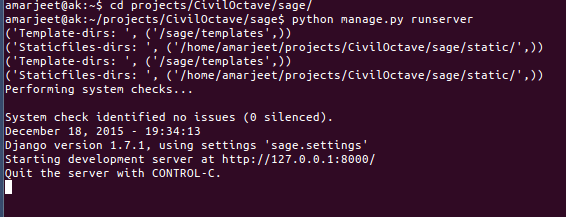
\includegraphics[scale=0.5]{images/out.png}
\caption{Output of runserver}
\end{figure}

\subsection{Database setup}
In this, we need to edit the settings.py file of the Project, that is the 
configuration file. It's a normal Python module with module-level 
variables representing Django settings. Change the following keys in 
the DATABASES 'default' item to match your database connection 
settings.
\begin{itemize}
\item ENGINE -- Either `django.db.backends.postgresql\_psycopg2', 
`django.db.backends.mysql',\\ `django.db.backends.sqlite3' or 
`django.db.backends.oracle'. Other backends are also available.
\item NAME -- The name of your database. If you're using SQLite, 
the database will be a file on your computer; in that case, NAME 
should be the full absolute path, including filename, of that file. If 
the file doesn't exist, it will automatically be created when you 
synchronize the database for the first time (see below). When specifying 
the path, always use forward slashes, even on Windows 
(e.g. C:/homes/user/mysite/sqlite3.db). 
\item USER -- Your database username (not used for SQLite).
\item PASSWORD -- Your database password (not used for SQLite).
\item HOST -- The host your database is on. Leave this as an empty 
string if your database server is on the same physical machine (not 
used for SQLite).
\end{itemize}

If you're new to databases, we recommend simply using SQLite by setting 
ENGINE to \\`django.db.backends.sqlite3' and NAME to the place where 
you'd like to store the database. SQLite is included as part of Python 
2.5 and later, so you won't need to install anything else to support 
your database.

While you're editing settings.py, set TIME\_ZONE to your time zone. The 
default value is the Central time zone in the U.S. (Chicago).

Also, note the INSTALLED\_APPS setting toward the bottom of the file. 
That holds the names of all Django applications that are activated in 
this Django instance. Apps can be used in multiple projects, and you 
can package and distribute them for use by others in their projects.

By default, INSTALLED\_APPS contain the following apps, all of which 
come with Django:
\begin{itemize}
\item django.contrib.auth -- An authentication system.
\item django.contrib.contenttypes -- A framework for content types.
\item django.contrib.sessions -- A session framework.
\item django.contrib.sites -- A framework for managing multiple sites 
with one Django installation.
\item django.contrib.messages -- A messaging framework.
\item django.contrib.staticfiles -- A framework for managing static 
files.
\end{itemize}

These applications are included by default as a convenience for the 
common case.

Each of these applications makes use of at least one database table, 
though, so we need to create the tables in the database before we can 
use them. To do that, run the following command:\\

	\$ python manage.py syncdb\\

The syncdb command looks at the INSTALLED\_APPS setting and creates 
any necessary database tables according to the database settings in 
your settings.py file. You'll see a message for each database table it 
creates, and you'll get a prompt asking you if you'd like to create a 
superuser account for the authentication system. Go ahead and do that.



\section{Introduction to Doxygen}
\section{Introduction to Doxygen}
\begin{figure}[h]
\centering 
\includegraphics[scale=1.3]{images/Doxygen.png}
\caption{Doxygen Logo}
\end{figure}
\noindent Doxygen is a documentation generator, a tool for writing software reference 
documentation. The documentation is written within code, and is thus 
relatively easy to keep up to date. Doxygen can cross reference 
documentation and code, so that the reader of a document can easily 
refer to the actual code.

Doxygen supports multiple programming languages, especially C++, C, 
C\#, Objective-C, Java, Python, IDL, VHDL, Fortran and PHP.[2] Doxygen
 is free software, released under the terms of the GNU General Public 
License.\\

\subsection{Features of Doxygen}
\begin{itemize}
\item Requires very little overhead from the writer of the documentation. 
Plain text will do, Markdown is support, and for more fancy or structured 
output HTML tags and/or some of doxygen's special commands can be used.
\item Cross platform: Works on Windows and many Unix flavors (including 
Linux and Mac OS X).
\item Comes with a GUI frontend (Doxywizard) to ease editing the options 
and run doxygen. The GUI is available on Windows, Linux, and Mac OS X.
\item Automatically generates class and collaboration diagrams in HTML 
(as clickable image maps) and $\mbox{\LaTeX}$ (as Encapsulated PostScript 
images).
\item Allows grouping of entities in modules and creating a hierarchy 
of modules.
\item Doxygen can generate a layout which you can use and edit to change 
the layout of each page.
\item Can cope with large projects easily.
\end{itemize}
\subsection{Installation of Doxygen}
Doxygen can be installed using following commands:\\

\hspace{4pt} \$ git clone https://github.com/doxygen/doxygen.git

\hspace{4pt} \$ cd doxygen

\hspace{4pt} \$ ./configure

\hspace{4pt} \$ make

\begin{figure}[H]
\centering 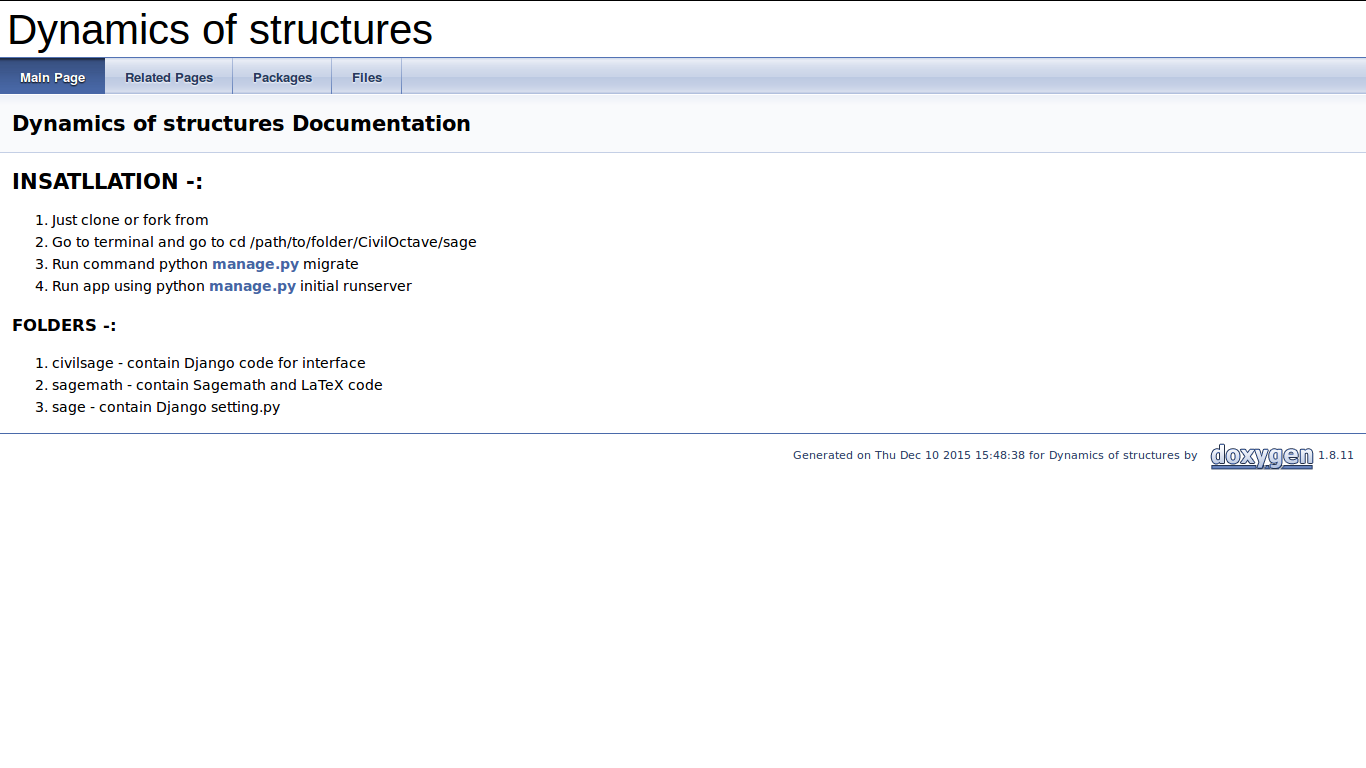
\includegraphics[scale=.35]{images/doc.png}
\caption{Documentation using Doxygen (main page)}
\end{figure}


\begin{figure}[H]
\centering 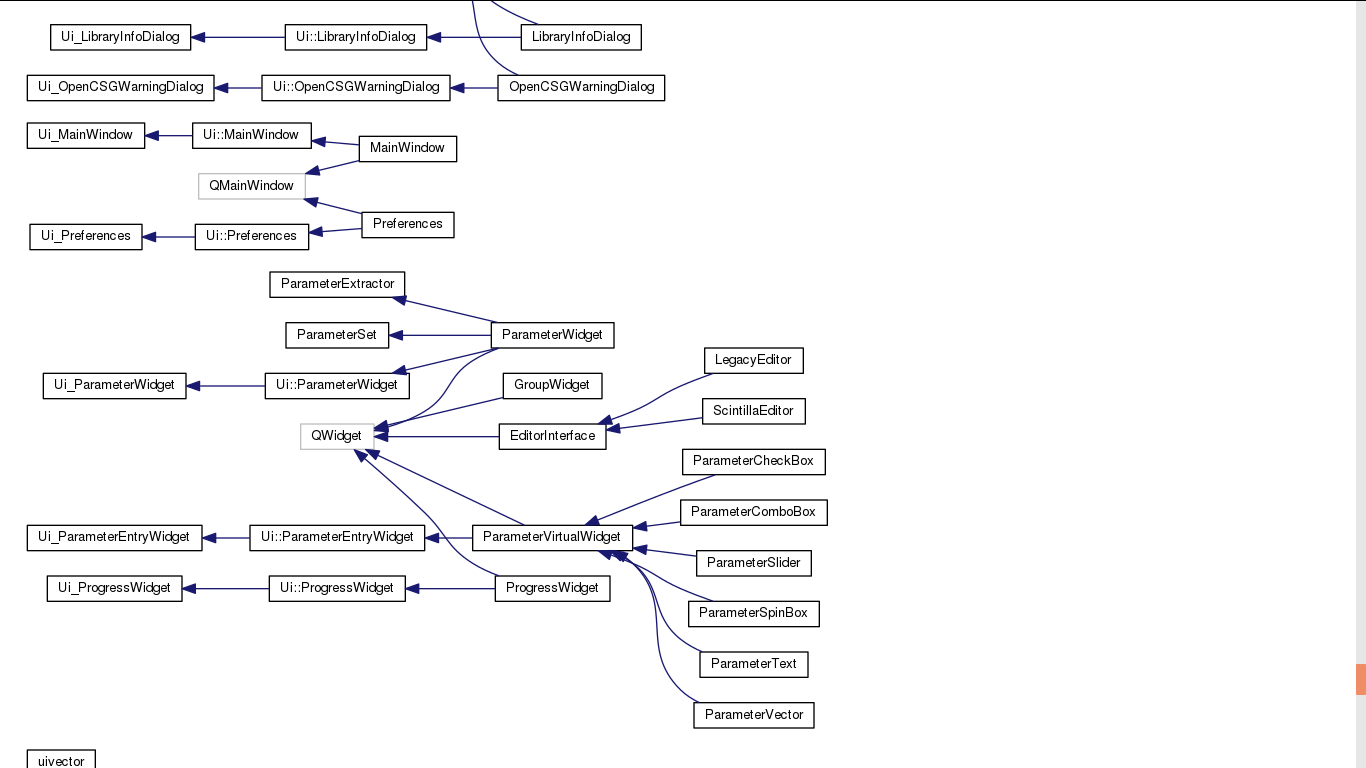
\includegraphics[scale=.35]{images/doc1.png}
\caption{Doxygen documentation of a function}
\end{figure}
\begin{figure}[H]
\centering 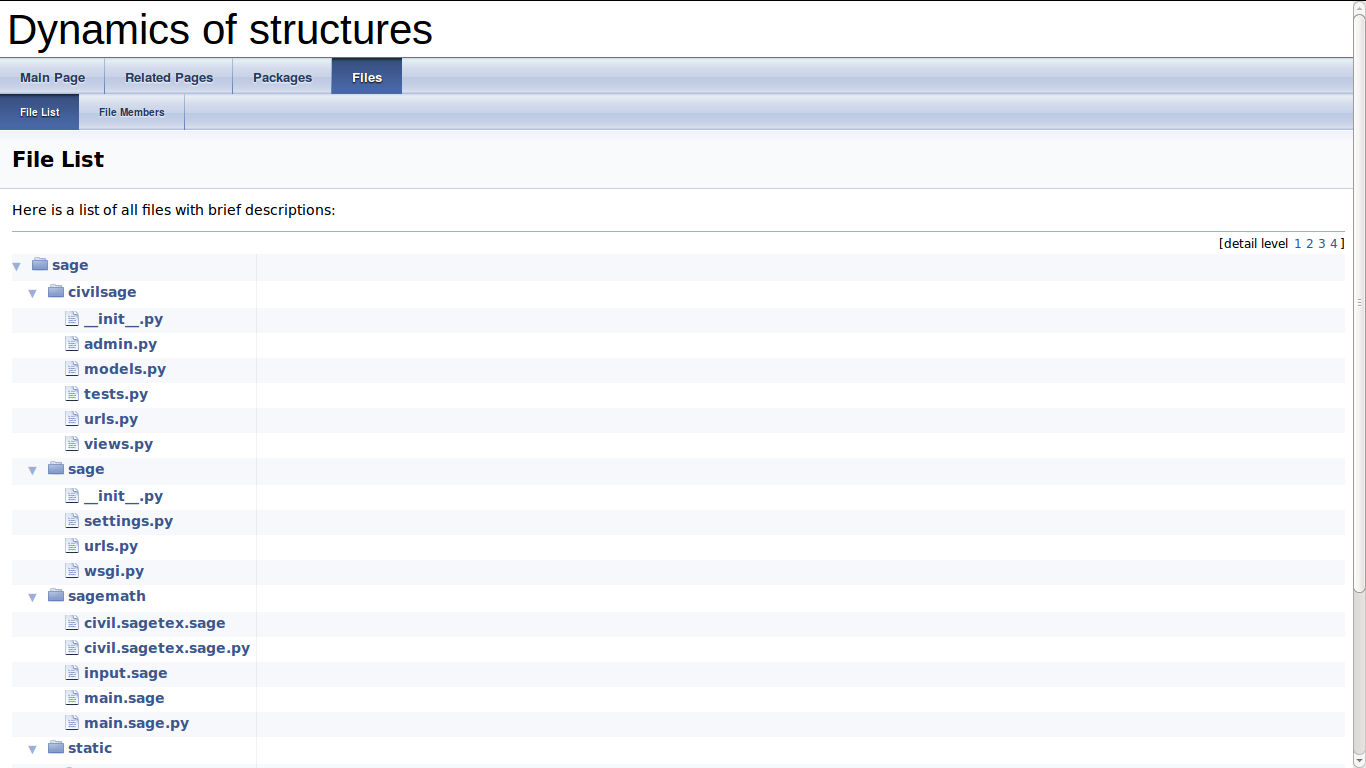
\includegraphics[scale=.35]{images/doc2.png}
\caption{Documentation using Doxygen(list of files)}
\end{figure}





\section{Introduction to Github}
\begin{figure}[!ht]
\centering

\includegraphics[width=0.3\textwidth]{images/github.png}                   
\caption{Github Logo}
\hspace{-1.5em}
\end{figure}
\leavevmode\\
GitHub is a Git repository web-based hosting service which offers all of the functionality of Git as well as adding many of its own features. Unlike Git which is strictly a command-line tool, Github provides a web-based graphical interface and desktop as well as mobile integration. It also provides access control and several collaboration features such as wikis, task management, and bug tracking and feature requests for every project.\\

GitHub has become such a staple amongst the open-source development community that many developers have begun considering it a replacement for a conventional resume and some employers require applications to provide a link to and have an active contributing GitHub account in order to qualify for a job.\\

The Git feature that really makes it stand apart from nearly every
other Source Code Management (SCM) out there is its branching model.\\
\\
Git allows and encourages you to have multiple local branches that can
be entirely independent of each other. The creation, merging, and
deletion of those lines of development takes seconds.\\ \\
This means that you can do things like:
\begin{itemize}
\item Frictionless Context Switching.\\ Create a branch to try out an
idea, commit a few times, switch back to where you branched from,
apply a patch, switch back to where you are experimenting, and merge
it in.
\item Role-Based Code lines. \\ Have a branch that always contains only
what goes to production, another that you merge work into for testing,
and several smaller ones for day to day work.
\item Feature Based Work flow. \\ Create new branches for each new
feature you're working on so you can seamlessly switch back and forth
between them, then delete each branch when that feature gets merged
into your main line.
\item Disposable Experimentation.\\  Create a branch to experiment in,
realize it's not going to work, and just delete it - abandoning the
work—with nobody else ever seeing it (even if you've pushed other
branches in the meantime).
\end{itemize}
Notably, when you push to a remote repository, you do not have to push
all of your branches. You can choose to share just one of your
branches, a few of them, or all of them. This tends to free people to
try new ideas without worrying about having to plan how and when they
are going to merge it in or share it with others.\\ \\
There are ways to accomplish some of this with other systems, but the
work involved is much more difficult and error-prone. Git makes this
process incredibly easy and it changes the way most developers work
when they learn it.

\subsection{What is Git?}
\begin{figure}[!ht]
\centering

\includegraphics[width=0.3\textwidth]{images/git.png}                   
\caption{Git Logo}
\hspace{-1.5em}
\end{figure}
Git is a distributed revision control and source code management (SCM) system with an emphasis on speed, data integrity, and support for distributed, non-linear workflows. Git was initially designed and developed by Linus Torvalds for Linux kernel development in 2005, and has since become the most widely adopted version control system for software development.\\

As with most other distributed revision control systems, and unlike most client–server systems, every Git working directory is a full-fledged repository with complete history and full version-tracking capabilities, independent of network access or a central server. Like the Linux kernel, Git is free and open source software distributed under the terms of the GNU General Public License version 2 to handle everything from small to very large projects with speed and efficiency.\\

Git is easy to learn and has a tiny footprint with lightning fast performance. It outclasses SCM tools like Subversion, CVS, Perforce, and ClearCase with features like cheap local branching, convenient staging areas, and multiple workflows.\\


\subsection{Various Git Commands}

Git is the open source distributed version control system that facilitates GitHub activities on your laptop or desktop. The commonly used Git command line instructions are:-\\

\begin{description}

\item [\$ git init [ project-name]]\\
Creates a new local repository with the specified name
\item [\$ git clone [url]]\\
Downloads a project and its entire version history\\
\item [\$ git merge [bookmark]/[branch]]\\
Combines bookmark’s branch into current local branch

\item [\$ git push [alias][branch]]\\
Uploads all local branch commits to GitHub

\item [\$ git pull] \leavevmode \\
Downloads bookmark history and incorporates changes

\item [\$ git add [file]]\\
Snapshots the file in preparation for versioning

\item [\$ git reset [file]]\\
Unstages the file, but preserve its contents

\item [\$ git commit -m "[descriptive message]"]\\
Records file snapshots permanently in version history\\

\end{description}

\section{SageMath}

\begin{figure}[!ht]
\centering

\includegraphics[width=0.7\textwidth]{images/sage.png}                   
\caption{SageMath Logo}
\hspace{-1.5em}
\end{figure}

SageMath (previously Sage or SAGE, System for Algebra and Geometry Experimentation) is mathematical software with features covering many aspects of mathematics, including algebra, combinatorics, numerical mathematics, number theory, and calculus.


The first version of SageMath was released on 24 February 2005 as free and open source software under the terms of the GNU General Public License, with the initial goals of creating an "open source alternative to Magma, Maple, Mathematica, and MATLAB". The originator and leader of the SageMath project, William Stein, is a mathematician at the University of Washington.


SageMath uses the Python programming language, supporting procedural, functional and object-oriented constructs.


\subsection{Features}
The Sage notebook document interface in a web browser.
Equation solving and typesetting using the SageMath notebook web interface


Features of SageMath include:
\begin{itemize}
\item  A browser-based notebook for review and re-use of previous inputs and outputs, including graphics and text annotations. Compatible with Firefox, Opera, Konqueror, Google Chrome and Safari. Notebooks can be accessed locally or remotely and the connection can be secured with HTTPS.
\item   A text-based command-line interface using IPython
\item   Support for parallel processing using multi-core processors, multiple processors, or distributed computing
\item   Calculus using Maxima and SymPy
\item   Numerical linear algebra using the GSL, SciPy and NumPy
\item   2D and 3D graphs of symbolic functions and numerical data
\item   Matrix manipulation, including sparse arrays
\item  Multivariate statistics libraries, using R and SciPy
\item A toolkit for adding user interfaces to calculations and applications
\item Graph theory visualization and analysis tools
\item Libraries of number theory functions
\item Support for complex numbers, arbitrary precision and symbolic computation
\item Technical word processing including formula editing and embedding SageMath within LaTeX documents
\item The Python standard library, including tools for connecting to SQL, HTTP, HTTPS, NNTP, IMAP, SSH, IRC, FTP and others
\item Interfaces to some third-party applications like Mathematica, Magma, R, and Maple
\item Documentation using Sphinx
\item An automated test-suite
\item Execution of Fortran, C, C++, and Cython code
\item Although not provided by SageMath directly, SageMath can be called from within Mathematica as is done in this Mathematica notebook example
\end{itemize}

\subsection{Installation From Source Code}
Steps for install SageMath -:
\begin{itemize}
\item	sudo apt-get install g++ lrzip
\item	lrunzip  "Downloaded-Zip-file".tar.lrz
\item	sudo apt-get dpkg-dev
\item	cd sageL
\item	sudo apt-get install binutils gcc make m4 perl tar
\item	sudo apt-get install build-essential m4
\item	export MAKE='make -j8'
\item	sudo apt-get install tk8.5-dev
\item	cd sage-directory
\item	./configure
\item	make
\end{itemize}



\section{Implementation}
\section{Implementation}
\begin{figure}[H]
    \centering 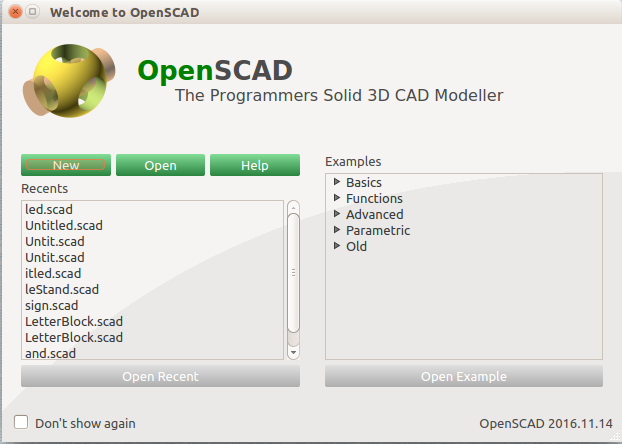
\includegraphics[width=0.7\linewidth]{images/output/1.png}
    \caption{StartUp Screen for OpenSCAD}
    \label{fig:1}
\end{figure}
\subsection{Multithreading}
In order to understand how we have attempted to implement multithreading for geometric rendering we need to understand the problem in substantial detail.\\
Even though it has been mentioned before profoundly, we feel the need the reiteration of what OpenSCAD is and how it achieves its goals. OpenSCAD is a 3D modeler i.e. it creates 3D models. The user interaction is done through a scripting language. This language describes the object(s) that the user wishes to create. This system has been put in place for the following reasons:
\begin{itemize}
	\item The fundamental geometric constructs of general purpose programming languages are too complex for an avergae computer user to learn and master. Even though ultimately, these constructs are being used to make everything in OpenSCAD but it is very difficult to expose the user to such tools. They are a little too fundamental and esoteric for the software to be of any help to your average modeler or designer who are unlikely to have much expertise of computer programming.\\
	That is why it becomes very important that the user is given an interface which has much less steeper learning curve than direct usage of geometric libraries. The OpenSCAD modelling language is just the interface for the job.
	\item Freedom and flexibilty of designing can be greatly compromised if only GUI constructs are used for modelling purpose. It is essential to give the user enough power to create complex and intricate designs easily without havnig to be limited by what the GUI has to offer. The modelling language, while being very intuitive is in fact very powerfull. The learning curve is much more user friendly without compromising the user's ability to make powerful designs. It saves a lot of time to use a higher abstraction of geometric constructs than to use the fundamentals them selves.\\
	The OpenSCAD modelling language thrives for the reasons any high level language thrives over a more machine related language. Time and effort of the programmer is saved and readability, portability are gained.
\end{itemize}
Here is a snapshot of the a model description using the above mentioned langauage:
\begin{figure}
    \centering 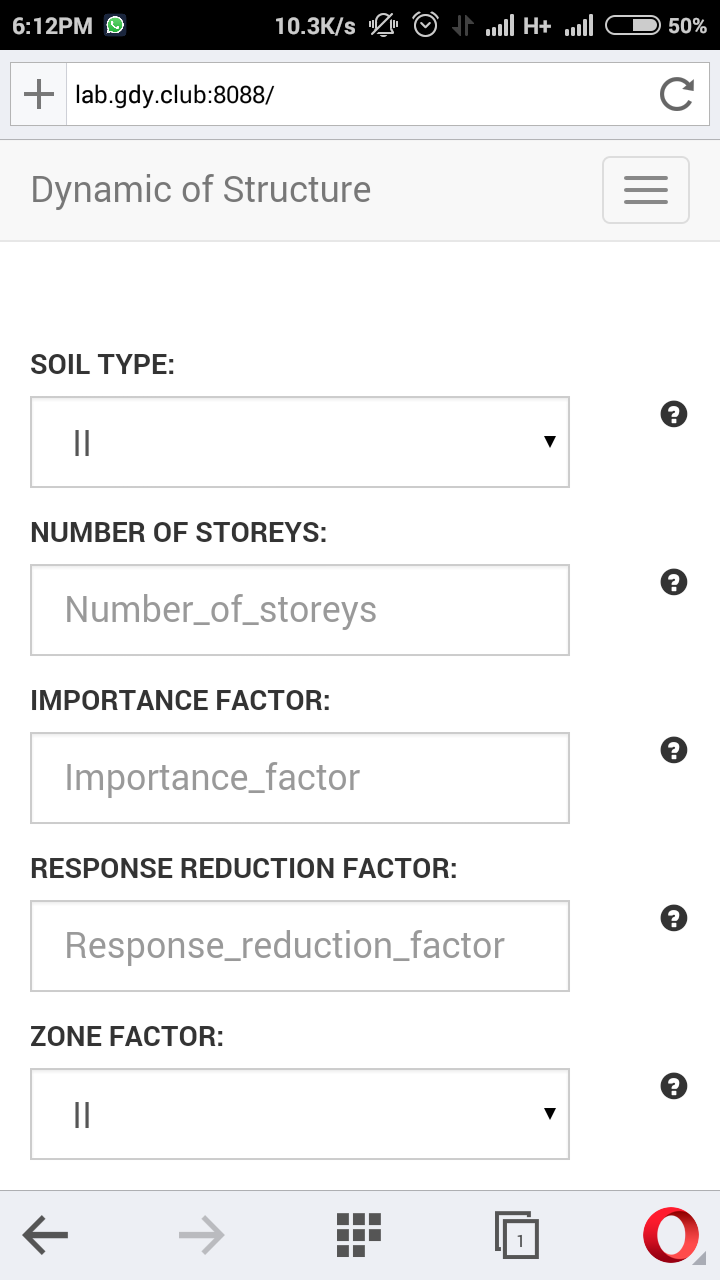
\includegraphics[width=\linewidth]{images/output/5.png}
    \caption{Working example of OpenSCAD}
    \label{fig:1}
\end{figure}
This language is parsed and converted into an Abstract Syntax Tree. This AST is used to turn descriptions of the objects into their graphic form. The AST is fed to an evaluator which reads the entire abstract syntac tree and turn it into a nodal tree. Each node in the tree represents geometric forms to be drawn. Once the node tree has been generated, references of this are pased around in order to accomplish various things. The same node tree can be used to generate the preview of the model using CSG and the same node tree is used to render the model. All of this can be summarised by the following flow chart:
\begin{figure}
    \centering 
    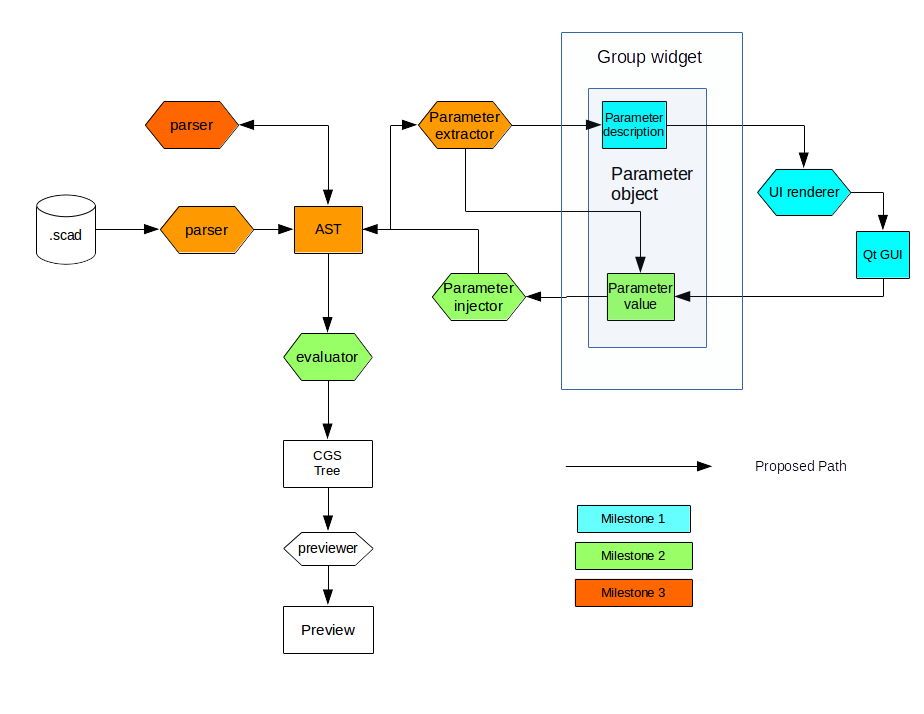
\includegraphics[width=\linewidth]{images/flowchart.png}
    \caption{Working flow of OpenSCAD}
\end{figure}
The first thing that was needed to be done was understanding the flow of the software and figuring out what sections of code needs to be parallelized. After forming a firmer understanding of the problem, it was required to check all the relevant data structures involved in evaluating the tree nodes. It was also be checked if any data structures used were needed to be modified or not. After fixing the appropriate data structures, all the feasible and plausible approaches were to be explored. Each approach has been evaluated on its merits and feasibility. Among all the options the one which is works well across all platform has been chosen. It goes without saying that the chosen solution has to meet all the requirement and implement the solution efficiently. After going through all of this the implementation began. The diagram below depicts the intended approach:
\begin{figure}
    \centering 
    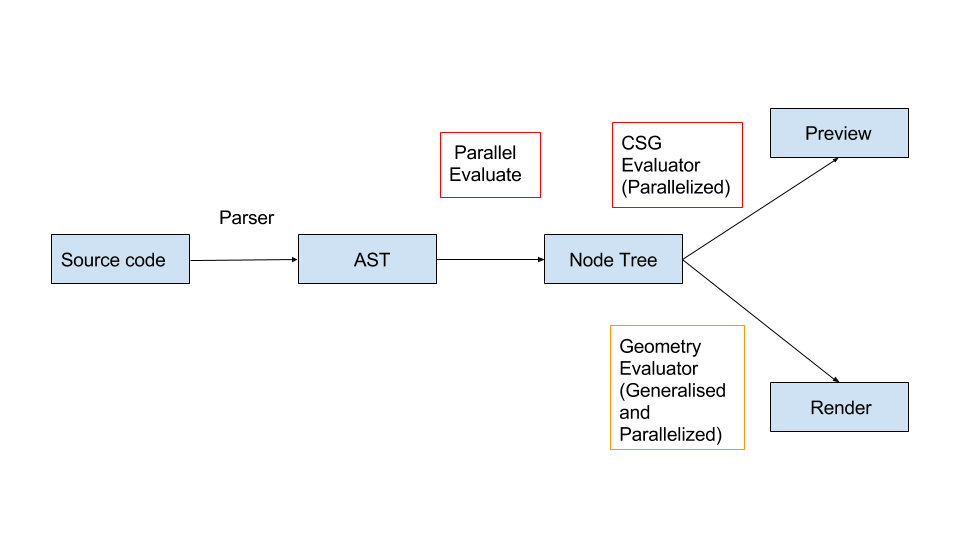
\includegraphics[width=\linewidth]{images/finalflow.png}
    \caption{Flowchart for the solution}
\end{figure}
During the implementation it was important to understand how the code works otherwise it will not have been possible to alter that code or even add to it. As OpenSCAD's GUI opens up, the code in the MainWindow.cc file is run. From here, the user can do many things but for our intent we are only going to focus on what happens when F6 is pressed. F6 is to issue the render command which is carried out via the actionRender() function. Following the flow of code from this function, it was descovered that the node tree is getting traversed recursively using the traverse function defined in the nodeVisitor.cc file. As mentioned, this function traverses each node is the node tree starting from the root node and then visiting each node recursively. Together with visiting each node, this function also calls out the accept() function on each node which is used to process the node further.\\
The whole point of multithreading was to parallelise this process of evaluating nodes. In its fundamental form, this is problem of applying parralelism to tree traversal. This parralelism can be achieved by simplying creating a new thread each time a new branch of the tree is to be traversed. But one may see, that this approach is not thread safe. First of all, the nodes that are getting visited must be accounted for in some sort of collection. And if various threads are going to visit the nodes and then update this collection then it becomes very important to make sure that no two threds are ever in a race, competing to update the collection at the same time. Such safety can be achieved by using lock mechanism.\\
This is not even the major problem, the real issue is in making sure that the global resources used by these functions are not unsafe from race conditions or concurrent access. Dealing with this took great effort and careful programming.
\subsection{Halting Mechanism for Render}
Ones the render process has been started, intentionally or unintentionally, there is nothing that can be done to stop the process without closing openSCAD altogether. The rendering process is not instantaneous making this a certain problem. There has to be method that on the user's command can halt an ongoing render process.\\
It is not just that the rendering process is to be stopped, it is also important to somehow perserve the partial work that has been done the rendering process before being halted by the user. This is achieved by caching the work and keeping the cache accesible across compiles in ordet to save time.\\
On carefull examination of the code, it was found that the cancel button was already part of the GUI. It just wasn't doing much usefull stuff to cancel the process. The cancel button is part of the progress widget GUI. And it is required to do is set a boolean variable to true. The variable name is wasCancelled. There is also function that checks the value of this variable to tell whether the process was cancelled or not i.e. the button was pressed or not. This function name is wasCancelled().\\
It is easy see that most pieces of the puzzle are already there. It is just required to place them properly and make them come together.\\
On some rigorous source browsing and consultation with the OpenSCAD developers, it was found that the assignment to true of the variable wasCancelled actually throws a programmer made exception: ProgressCancelException. Our job was to ensure that proper action is taken when this exception is raised. To do so, we had to tweak the visit() function which is responsible for visiting each node in the tree. This function was not singular. There were any overloaded versions of this depending on the type of node being visited. Hence the same work had to be done for each node.\\
After visiting each node, a made to call to a reporting function was made to happen. This function basically communicates to the progress widget about the number of nodes visited by it. The progress bar ranges from 1 to 1000. But this is not the sole purpose of this function, it also check at the end whether the exception has been raised or not. If it finds the exception is raised, it sets in motion a sequence of function calls that lead to safe halt of the render process. The following figure shows the working of the progress report and the cancel button:
\begin{figure}
	\centering
	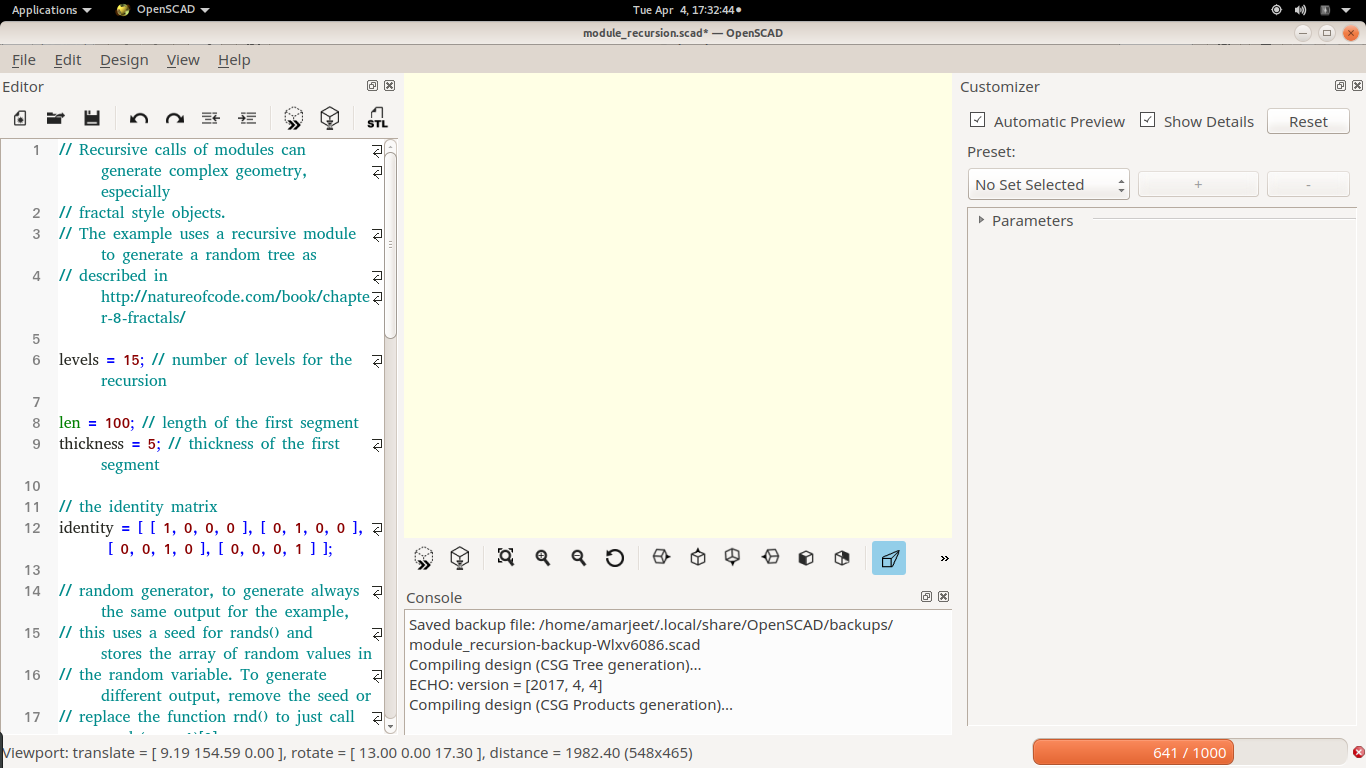
\includegraphics[width=\linewidth]{images/output/progress_widget.png}
	\caption{Progress Widget working}
\end{figure}
\subsection{Finding Root Tag Nodes}
3D models are often formed by taking two separate entities and then merging them using some of the operations like union, intersection and difference. All of this is taken care of at the back end using the node tree. In the node tree, one can have two separate entities as the child of a node and that node being the operation that is to be performed on those entities. As such, in the same model we can have various subsystem of nodes interacting with each other in order to give the final result. This just goes to show that subtrees within the node tree are very much capable of existing independantly. As such, sometimes it is desired by the user to only evaluate a certain branch of subtree of the whole tree. This means everything else in the tree except for that branch is useless for the time being. In order to save time and resources, we have to process and render only that subset.\\
The other parts of the tree are to be ignored. This certainly can not be done by commenting out, or deleting other nodes in the description of the language and then recompiling it. That approach would be very counterproductive.\\
A better way of doing this would be let the whole tree be in place. And when it is time to compile the part of the tree, simply tell the compiler to skip over to the subtree that is required and quit as soon as the compiler is done with that subtree. This way, nothing has to get deleted and only that part is compiled that is actually required. That is why there is a mechanism by which the user is allowed to set for a temporary period of time, a pseudo-root node. This root node can be anywhere in the tree. And when this is to be rendered, the software searches for it in the tree and returns a reference for it.\\
However, since the user is allowed to set multiple pseudo nodes in the tree, the searching function has to store references to all of them. Eventually only the first one of these stored references are used, but others are stored nonetheless. And if infact there are no such pseudo root nodes in the tree, then null is returned, indicating that the actuall root of the tree is to be treated as the root for the next render. It is important that we store all the nodes that have been marked as pseudo-roots. This marking is done by setting an attribute of each node to RootTag. This significanc stems from the fact that it is unnatural and hence useless to have multiple nodes as pseudo roots. For this reason, the user must be reminded as to how many markers have been set. This reminder is given in the form of a warning. In the picture below, one can see how the system worked before:\\
\begin{figure}
	\centering
	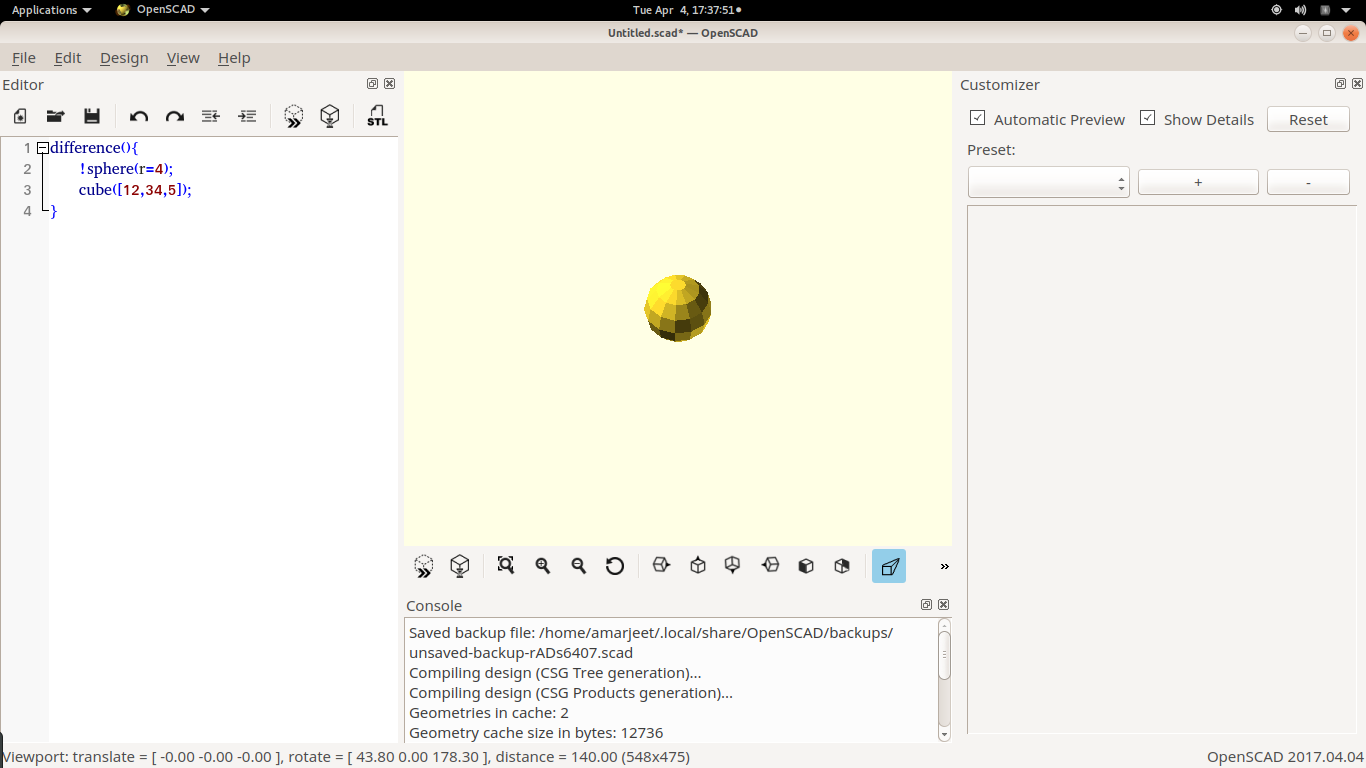
\includegraphics[width=\linewidth]{images/output/before_okay.png}
	\caption{Finding RootTag nodes previously}
\end{figure}
In this figure we can see how only one node has been marked as the pseudo root node (using the exclamation mark). And corresponding to it, we see no warnings because no warnings are due. But consider the following case:\\
\begin{figure}
	\centering
	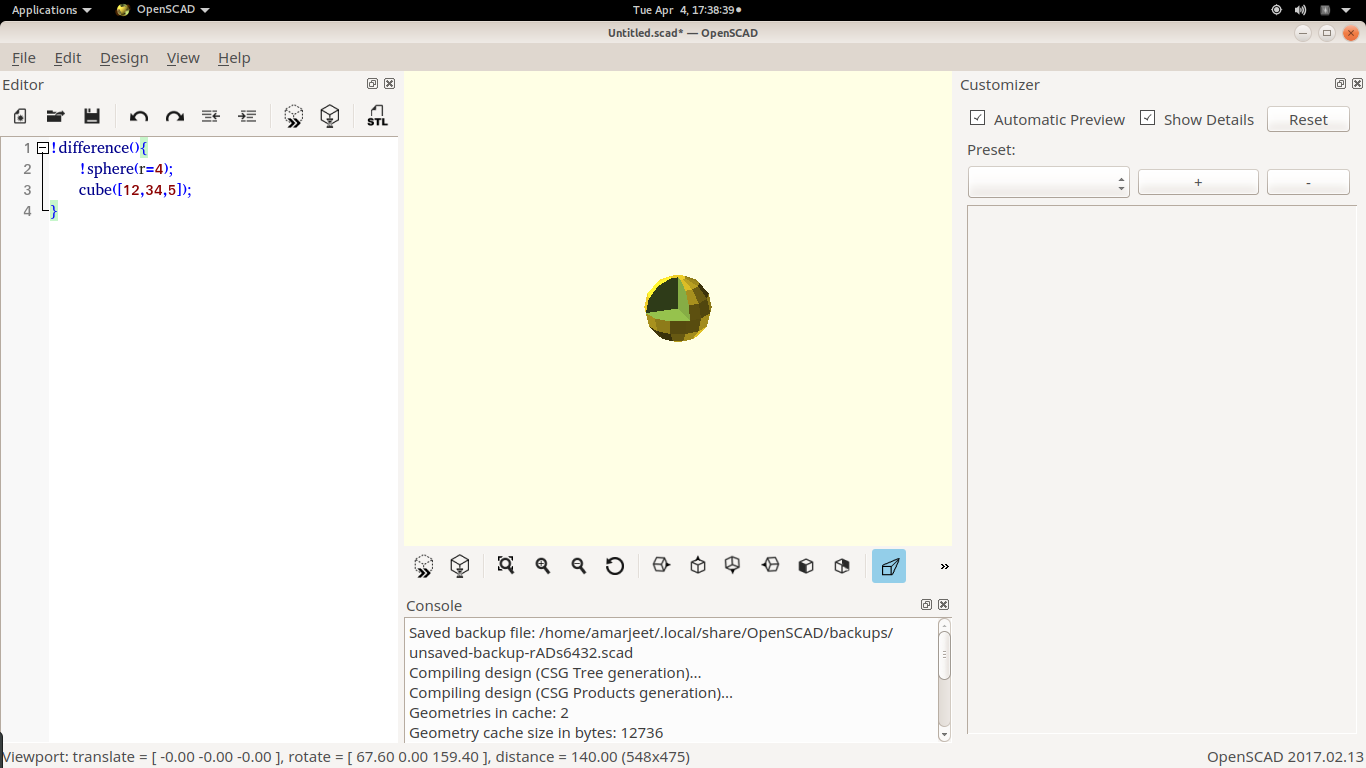
\includegraphics[width=\linewidth]{images/output/before_wrong.png}
	\caption{Finding multiple RootTag nodes previously}
\end{figure}
As seen, even though we had multilpe tags in the model, we didn't get any warnings.
The previous version of this function would search through the tree to find this tag. And the function would return as soon as it has found the first node with this tag or if it has exhausted the search space. In anycase, it was not possible to store all the nodes. We have implemented a solution to this problem by amending this search function.\\
In the present version of this function, we have implemented a lambda function. This lambda function recurses through the entire tree and checks to see if a node is marked or not. All the marked nodes are stored in vector. The result will still be the same as before because only the first element stored in the vector will be rendered, but atleast with this approach, the user is provided with a list of nodes that they have marked unnecessairily. The following figure shows how things are done now:\\
\begin{figure}
	\centering
	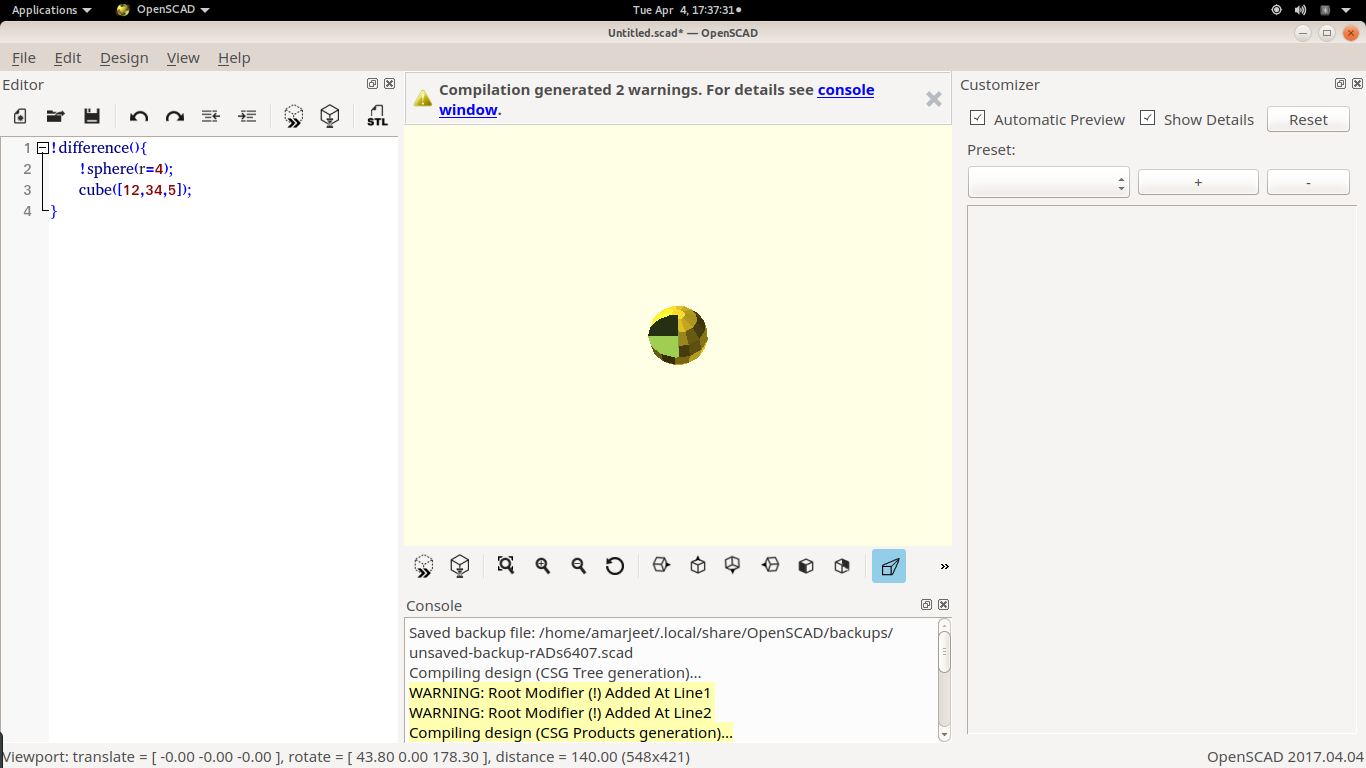
\includegraphics[width=\linewidth]{images/output/now_right.png}
	\caption{Finding multiple RootTag nodes now}
\end{figure}


\section{Testing}
Testing a program consists of providing the program with a set of test inputs (or test cases) and
observing if the program behaves as expected. If the program fails to behave as expected, then the
conditions under which failure occurs are noted for later debugging and correction. 


This software had been taken through rigorous test to fully found potential causes of error and system failure
and full focus have been given to cover all possible exceptions that can 
occur and cause failure of the software.
As this software is based on intensive background process it have been taken care that 
if correct input and email address are given then processing of user job can even continue or a least automatically 
restart even after server shuts down or even crash.

Following is data collected Table no. \ref{table} and corresponding Graph figure \ref{fig:graph} for analyzing the computation time taken by software 
to its maximum supported value at this time-:
\begin{sagesilent}
list=((5,0.341143),(
10,1.768803),
(15,5.827224),(
20,35.870348),(
30 ,111.939167),(
40 ,484.906122),(
50,1527.764697))
r = [(list[i][0],list[i][1]) for i in range(7)]
p=list_plot(r,color='red',plotjoined=True,marker=".",frame=True,axes_labels=['$Number \ Of \ Storeys$ axis','$Time(sec)$ axis'],axes=False)
\end{sagesilent}

\begin{figure}[H]
	\sageplot[scale=0.75]{p}
	\caption{Time complexity graph of Dynamics of Structure}
	\label{fig:graph}
\end{figure}



\begin{table}[h]
\centering
\begin{tabular}{ ||c|c|| }
\hline
 \multicolumn{2}{||c||}{Time complexity analysis table} \\
 \hline
 Number of Storeys & Time(sec) \\ [0.5ex] 
 \hline \hline
	5 & 0.341143 \\ \hline
	10 & 1.768803 \\ \hline
	15 & 5.827224 \\ \hline
	20 & 35.870348 \\ \hline
	30 & 111.939167 \\ \hline
	40 & 484.906122 \\ \hline
	50 & 1527.764697 \\ [1ex]
 \hline
\end{tabular}
\caption{Computational analysis of DoS}
\label{table2}
\end{table}

\begin{table}[h]
\centering
\resizebox{\textwidth}{!}{\begin{tabular}{ |c|c|c|c| }
\hline
 \multicolumn{4}{|c|}{Test cases for main page(index.html) } \\[0.5ex]
 \hline
 Input & Desired Output & Actual Output & Status \\ [0.5ex] 
 \hline \hline
 Inputs range exceeds & Alert user,Don't proceed & Alert user,Don't proceed. & Pass\\ \hline
 Any one or more field left empty & Alert user about range. Don't proceed & Alert user about range. Don't proceed & Pass\\ \hline
 CSV selected: No & Direct to manual fill of matrices & Direct to manual fill of matrices & Pass\\ \hline
 CSV selected: Yes & Direct to uploading of file & Direct to uploading of file & Pass\\ \hline
 Email selected: Yes & Show email field after Submit & Show email field after Submit & Pass\\ \hline
 Email selected: No & Proceed without email & Proceed without email & Pass\\ \hline
 Help pressed  & Show Detailed user help & Show Detailed user help  & Pass\\ \hline
 Autofill values & Automatically fill default values & Automatically fill default values & Pass\\ \hline
 
\end{tabular}}



\caption{Computaional anaysis of DoS}
\label{table3}
\end{table}

\begin{table}[h]
\centering
\resizebox{\textwidth}{!}{\begin{tabular}{ |c|c|c|c| }
\hline
 \multicolumn{4}{|c|}{Test cases for manual fill(matrix.hmtl) } \\[0.5ex]
 \hline
  Input & Desired Output & Actual Output & Status \\ [0.5ex] 
 \hline \hline 
 Email Address not filled & Give PDF after all processing & Give PDF after all processing & Pass\\ \hline
 Email Address filled and Submit & Show message, redirect to homepage & Show message, redirect to homepage & Pass\\ \hline
 Input range exceeds or not filled & Show error message & Show error message & Pass\\ \hline

\end{tabular}}



\caption{Tests for manual fill}
\label{table4}
\end{table}


\begin{table}[h]
\centering
\resizebox{\textwidth}{!}{\begin{tabular}{ |c|c|c|c| }
\hline
 \multicolumn{4}{|c|}{Test cases for file fill(file.html) } \\[0.5ex]
 \hline
 Input & Desired Output & Actual Output & Status \\ [0.5ex] 
 \hline \hline 
 Email Address not filled & Give PDF after all processing & Give PDF after all processing & Pass\\ \hline
 Email Address filled and Submit & Show message, redirect to homepage & Show message, redirect to homepage & Pass\\ \hline
 Input range exceeds or not filled & Show error message & Show error message & Pass\\ \hline
 Wrongly formatted CSV file & Give error message with Possible errors  & Give error message with Possible errors & Pass\\ \hline
\end{tabular}}
\caption{Tests for csv upload page}
\label{table5}
\end{table}


\begin{table}[h]
\centering
\resizebox{\textwidth}{!}{
\begin{tabular}{ |c|c|c|c| }
\hline
 \multicolumn{4}{|c|}{Test cases for possible source of problems } \\[0.5ex]
 \hline
  Input & Desired Output & Actual Output & Status \\ [0.5ex] 
 \hline \hline 
 URL refreshed & Send to homepage & Send to homepage & Pass\\ \hline
 server stops or rebooted & Start processing interrupted requests & Start processing interrupted requests & Pass\\ \hline
\end{tabular}}



\caption{Test case (general)}
\label{table}
\end{table}



\chapter{CONCLUSION AND FUTURE SCOPE}
\section{Conclusion}
DoS is a very efficient application which help in generating result for analysis of structures. It
can be used by Civil Engineers and M.Tech. students and even layman. It's less time consuming and user-friendly which let the User work in batch mode 
and free him from all the installation process. It is a web application that can be accessed from a number of devices. The responsive User Interface makes it easy for the users to operate it. Many efforts were made to ease the usage for the users. Hence, it is expected to be work properly in different conditions. But any future bug reports or improvements are always welcomed and will be processed happily.

I learn a lot by working on this project. During this period I got to learn a vast number of
technologies. These are listed below:
Operating system: Ubuntu
Language used: Python, HTML, CSS, shellscript
Framework: Django
Technogloy: \LaTeX{}, Djanog, Doxygen, Sagemath, Git 
So during this project I learn  all the above things. Above all I got to know how software is
developed and how much work and attention to details is required in building even the most basic
of components of any project. Planning, designing, developing code, working in a team, testing,
etc. These are all very precious lessons in themselves.
Aside from all above I got go know about various methods like -:
\begin{enumerate}
\item Threading the programs 
\item Embedding and using different tech in one software.
\item How to work like in group for development of software.
\item How to apply juggaar(innovated) in softwares to get problem solved. 
\end{enumerate}

Beside these technology used in project I also get to know some other tech also like -:
\begin{enumerate}
\item  OpneCV (image processing)
\item opensshserver 
\item reveal.md, impress.js (for making presentations)
\end{enumerate}  



\section{Future Scope}
OpenSCAD being a open source project and supported by a large open Soure community have a lot of scope for future improvements and additions as other individuals can also contibute in it and add additional functionality. One of the example is my project only customizer for OpenSCAD.

Being a Open Soucre project their is constant flow of suggestion and demands by people for additional functionality and improvment in exiting features.
Customizer being no expection constant flow of feature of suggestions and feature requests even before the start of development. Her is small list of the Features that would be added in near future.

\begin{enumerate}

\item \textbf{Adding support for InBuid syntax:} It was decided much at beginning of the project that this feature will be ported using a special syntax then relying on the comment based syntax. Discussion has been going on related to deciding the syntax for customizer.   

\item \textbf{Option to Add images:} It have been proposed that their should be feature to add images through customizer.  

\item \textbf{Option to Include files with Customizer:} This feature will help people change the include file with the help of Customizer which could provide feature which would be related to Run Time Polymorphism.

\item \textbf{Conditional display of Parmaeter is customizer:} Sometime people want to show different set of parmaters based on the chooses made by user before that parameter or sometime we just want to hide the parameters because of selection made by user in pervious parameter.

\item \textbf{Improving GUI part:} There have been some suggestions related to improving the GUI of the Customizer
https://github.com/openscad/openscad/issues/1845 . 
\item \textbf{Providing syntax to manuplate modules parameter:} This feature will help user pick a customizer version of the module using the customizer. They will be able to Customize the parameters of modules using and the Customizer than drag that in to the file to call it with customized parameter.
\end{enumerate} 

Apart from these features their are Some suggestion related to how existing feature would be improved to refer to that you can visit following: 

\begin{enumerate}
	\item https://github.com/openscad/openscad/issues/1844
	\item https://github.com/openscad/openscad/issues/1840
	\item https://github.com/openscad/openscad/issues/1781
	\item https://github.com/openscad/openscad/issues/722
\end{enumerate} 

\begin{thebibliography}{9}
\bibitem{} Dynamics of Structure(DoS), https://github.com/amarjeetkapoor1/CivilOctave
\bibitem{} \LaTeX{} https://www.sharelatex.com
\bibitem{} Sagemath www.sagemath.org/
\bibitem{} Django https://docs.djangoproject.com/
\bibitem{} Doxygen www.doxygen.org
\bibitem{} My Blog, https://amarjeetkapoor1.wordpress.com
\bibitem{} My Github Profile, https://github.com/amarjeetkapoor1
https://en.wikipedia.org/wiki/OpenSCAD
http://www.openscad.org/
http://customizer.makerbot.com/docs
https://amarjeetkapoor1.wordpress.com/2016/07/04/user-interface-for-customizing-models/
%http://www.openscad.org/news.html#20160714


logo

https://www.quora.com/Is-there-an-official-C++-logo

%https://en.wikipedia.org/wiki/GNU#/media/File:Heckert_GNU_white.svg

%https://en.wikipedia.org/wiki/Qt_(software)#/media/File:Qt_logo_2015.svg

%https://upload.wikimedia.org/wikipedia/commons/c/ce/Doxygen.png

%https://en.wikipedia.org/wiki/GitHub#/media/File:GitHub_logo_2013_padded.svg

%https://en.wikipedia.org/wiki/Git#/media/File:Git-logo.svg

%Published by the Free Software Foundation
%51 Franklin Street, Fifth Floor
%Boston, MA 02110-1301 USA
%Printed copies are available from the Free Software Foundation.
%ISBN 1-882114-44-2

%https://en.wikipedia.org/wiki/Qt_(software)

%https://en.wikipedia.org/wiki/C%2B%2B

%Flex/Bison Tutorial
%Aaron Myles Landwehr
%aron+ta@udel.edu

\end{thebibliography}

\end{document}

